%\documentclass{sigchi}
\documentclass{sig-alternate-10pt}


% llt: Define a global style for URLs, rather that the default one
%\makeatletter
%\def\url@leostyle{%
%  \@ifundefined{selectfont}{\def\UrlFont{\sf}}{\def\UrlFont{\small\bf\ttfamily}}}
%\makeatother
%\urlstyle{leo}


% To make various LaTeX processors do the right thing with page size.
\def\pprw{8.5in}
\def\pprh{11in}
\special{papersize=\pprw,\pprh}
\setlength{\paperwidth}{\pprw}
\setlength{\paperheight}{\pprh}
\setlength{\pdfpagewidth}{\pprw}
\setlength{\pdfpageheight}{\pprh}



\usepackage{graphicx}
\usepackage{epstopdf}
\usepackage{balance}
\usepackage{comment}
\usepackage{times,epsfig,subfigure,endnotes,color,url,paralist,multirow,float}
\usepackage[lined,ruled,linesnumbered,vlined]{algorithm2e}

% Make sure hyperref comes last of your loaded packages,
% to give it a fighting chance of not being over-written,
% since its job is to redefine many LaTeX commands.
\usepackage[pdftex]{hyperref}
\hypersetup{
    pdftitle={SIGCHI Conference Proceedings Format},
    pdfauthor={LaTeX},
    pdfkeywords={SIGCHI, proceedings, archival format},
    bookmarksnumbered,
    pdfstartview={FitH},
    colorlinks,
    citecolor=black,
    filecolor=black,
    linkcolor=black,
    urlcolor=black,
    breaklinks=true,
}

% create a shortcut to typeset table headings
\newcommand\tabhead[1]{\small\textbf{#1}}

\newcommand{\superscript}[1]{\ensuremath{^{\textrm{#1}}}}
\def\sharedaffiliation{\end{tabular}\newline\begin{tabular}{c}}

\def\winlab{\superscript{\dag}}
\def\cmu{\superscript{$\ast$}}
\def\ut{\superscript{\S}}
%\def\cornell{\superscript{$\star$}}

%\makeatletter
%\let\@copyrightspace\relax
%\makeatother


\begin{document}

\title{Whose Move is it Anyway? : Authenticating Smart Wearable Devices Using Unique Human Body Movement Patterns}

\numberofauthors{1}
\author{
\alignauthor
Sugang Li\winlab, Ashwin Ashok\cmu, Yanyong Zhang\winlab, Chenren Xu\cmu, Macro Gruteser\winlab\\
\vspace{4mm}
        \affaddr{{\winlab}WINLAB, Rutgers University, North Brunswick,NJ, USA}\\
          \vspace{1mm}
        \affaddr{{\cmu}Carnegie Mellon University, Pittsburgh, PA, USA}\\
}

\maketitle
% infer number of people, queue serving, traffic pattern,mood inference
% add comparison of time convergence of cell and point, RSS signatures for
%different phones, can we detect how many people when drive by? add wifi
%receiver part.
\newcommand{\systemname}{{\em Headbanger}}

\begin{abstract}
In this paper, we present the design, implementation and
user studies of a novel approach to authenticate
wearable devices users based on their unique behavioral patterns. We 
prototype an authentication system, dubbed {\em Headbanger} for
head-worn wearable devices by monitoring user's unique head-movement patterns 
in response to an external audio stimulus. 
Solutions today primarily rely on indirect authentication
mechanisms through the user's smartphone, which can be cumbersome and more 
susceptible to adversary intrusions. Biometric solutions, 
are subject to the availability of the specific sensors in the wearable unit. 
Using a head-worn personal imaging device as a running example and
through extensive experimental evaluation with 30 human subjects, we show
that our mechanism can authenticate users with an average true acceptance rate of
95.57\% while keeping the average false acceptance rate of 4.43\%.

\end{abstract} 

%The recent years have seen a significant growth in popularity of
%smart wearable devices. This growth can be attributed to the advances in
%hardware miniaturization technology as well as economically affordable
%and energy efficient sensing and computing. While size, energy and cost
%constraints remain key motives for improvements in wearable computers'
%design, the aspect of user authentication has received relatively less
%attention. Wearable devices often collect and store sensitive data about
%users, and thus there is an obvious need to authenticate the right user to the
%device.
\section{Introduction}\label{sec:intro}

We live in a world that has seen a generation of technological revolutions;
from wired to wireless communications, immovable to mobile machines, large
sized to hand-held devices. Today, we are witnessing what can be deemed as the
next phase of mobile revolution through {\em wearable computers}. Research in
wearable computers can be dated back to as early as 1980s when Steve Mann
developed a prototype heads-up-display goggles~\cite{mann1997wearable}. Thanks to the
advances in hardware miniaturization technology, cheap sensors/processor
chips, and low-power sensing/computing, today, wearables are available
off-the-shelf and have almost become an integral part of human
lives~\cite{googleglass,smartwatch,fitbit}.

%This is clearly evident from the surge in the number and types of wearables
%that are commercially available -- ranging from smart glasses, smart
%necklaces, smart wristbands, to smart watches.
The surge in wearables is clearly seen commercially through the array of
smart wearable devices seeping fast into the market. Research on wearables has
actively picked up and is progressing over the day. Keeping in mind the
resource limitations on wearable computers research so far has primarily
been addressing three key optimization parameters in
design: size, energy and cost. With the onset of proliferation of wearable
devices, in the recent times the aspect of security and privacy have also been
adding key concerns to wearable computer usage.
A solution for safeguarding the security and privacy of user's data on the
wearable device is only effective as long as the device itself is
authenticated to the right user/owner.

\begin{figure}
\centering
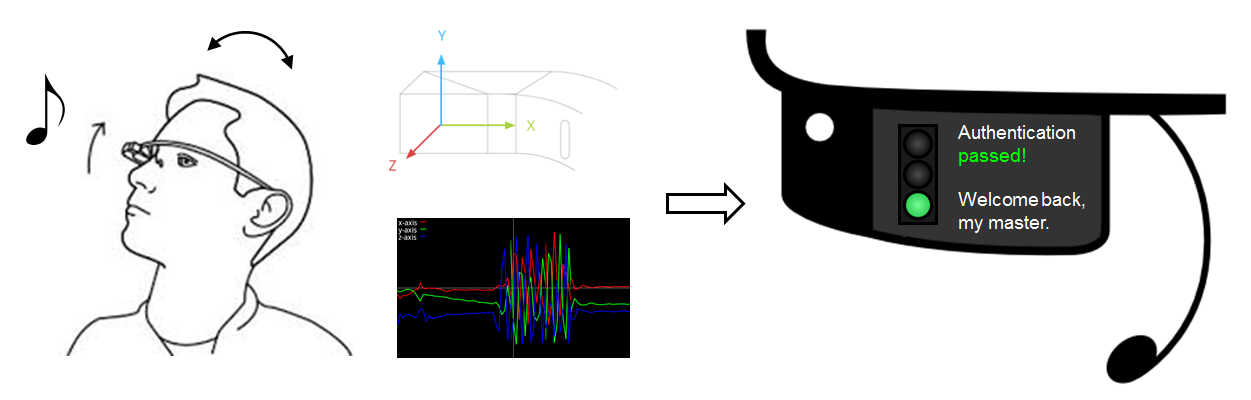
\includegraphics[width=\columnwidth]{fig/headbanger-illustrate.png}
\caption{Illustration of Headbanger. The head-worn device authenticates the
right user based on signatures generated from head-movement patterns in
response to an audio snapshot played on the device.}
\label{fig:headbanger-illustrate}
\end{figure}

\vspace{1mm}\noindent{\bf Authentication Challenge.}
%User-authentication for wearable devices has so-far received relatively less
%attention; commercially as well as in research.
Authentication on most commercially available wearable devices
today~\cite{fitbit, smartwatch} relies on an indirect mechanism, where users
can login to their wearables through their phones. This requires the wearable
device to be registered and paired to the user's mobile device, which makes it
inconvenient as the user has to carry both the devices. The security of this
approach is also in question as it increases the chance of hacking into
 both the devices if either of the devices are lost or stolen.
Some devices including Google Glass~\cite{googleglass} and
FitBit's health tracker~\cite{fitbit}, pair the device to the users email
account instead of the phone for user's convenience; however, it does not add any
security benefit. Though wearable devices today almost contain the same suite
of sensors as a smartphone, the computing capacity and battery lifetime of
wearables are far less comparable. This implies that, translating the same
 authentication solution from a phone to the wearable device, to enable
direct authentication, is not only undesirable but also impractical.
\emph{Thus, the need for the day is a simple, low-power, and accurate
direct authentication solution.}
%For example, fitness trackers and
%smart-watches are tethered to user's mobile device to connect to the
%Internet as well as for remote data collection.

There have also been a few specific point solutions that propose to directly
authenticate the user to the device using biometric signatures~\cite{rahman2014bodybeat,cornelius2014wearable}. However, collecting and recognizing these biometrics is subject
to the availability of the sensing hardware and the computing capability on
the wearable units, hence unrealistic in most
cases. The recent years have also seen a significant interest in using
behavioral characteristics of humans as biometric signatures for mobile phone
authentication~\cite{stevenage1999visual,okumura2006study,monrose2000keystroke,jorgensen2011mouse,bo2013silentsense,de2012touch}.
For example, human walking gait, arm swings, typing patterns, body pulse
beats, eye-blinks have all been found to be distinctive in human beings.
The main advantage of using behavioral biometrics is that the signatures can
be generated from raw data of basic sensor that are inbuilt in mobile phones
such as motion sensors, camera, microphones etc. However, what behavioral
biometric remains the best suited for a wearable device and if such a
biometric can be captured by the wearable device lays a fundamental question
for a system that may adopt this approach.

\vspace{1mm}\noindent{\bf Head-movement based authentication.}
In this paper, we propose to authenticate wearable devices to users based on
their unique behavioral patterns. Keeping in mind the feasibility of
implementation and the availability of the sensor on the wearable device,
we design a system that authenticates users to their device directly through
their head-movement patterns.
In particular, we prototype an authentication system, dubbed {\em Headbanger},
that generates a signature from user's head-movements that serves as the
behavioral biometric for authentication. To ensure that the user is proactive
in making head-movements we stimulate the process by playing a short duration
audio track with fast beats. The user in response to the rhythm and beats
makes head-movements that are captured by the accelerometer and processed to
generate and authenticate the user's unique biometric signature.
While we use a Google Glass a running example for the wearable device, our
design can be applied to other head-worn gadgets and any system that can
record head-movements through motion sensing.
Our choice for using head movements is motivated by the fact that head-worn
wearables are becoming very common today and such devices are already equipped
with motion sensors; for example, personal imaging and heads-up display
devices, gaming headsets, AI devices.

%Unlike physiological biometrics that require custom hardware,
%behavioral biometrics offer a much more available/conveient solution. The
%challenge, however,
%is to ensure that these patterns are repeatable under all circumstances that
%the user encounters as well as the differentiability factor between different
%human beings. %We show that by using the same external stimulus among all
%%users
%the baseline for comparison is achieved much easier and the head-patterns are
%more consistent and differentiable among users.

%Subconscious head-movement, or any body movement as a matter
%of fact, can be very random in general.
% Our design assumes that there is only one owner per glass, and we can easily
%extend our scheme to handle the cases with multiple owners.

In summary, the key contributions of this paper are:

\begin{enumerate}

\item We propose a technique for direct authentication to wearable devices
using head-movement patterns. We show that user's head-movement patterns
contain unique signatures that when inferred correctly can be used as valid
behavioral biometrics for authentication.

\item We design an authentication system, \systemname,~ that records,
processes, generates unique signatures, and classifies head-movement patterns
of users based on the accelerometer (inbuilt on the wearable device) sensor
readings.

\item We devise of a set of light-weight preprocessing and classification algorithms that can effectively transform raw and noisy sensor data into accurate authentication results. We aggressively optimize the processing latencies of these algorithms so that they are well suited for wearable devices.

\item We implement a data collection application on Google Glass that plays a
fast beat music (preloaded) through the Glass's speakers and simultaneously
records and filters accelerometer sensor data. We use this data collection app
in our experiments to evaluate the system.

\item Through extensive experiments involving multiple users\footnote{Our
human user experiments were approved by Rutgers University IRB} and over
different system design parameters we have shown that head-movement patterns
can be used as a
valid behavioral biometric.
To effectively identify a smart wearable device user,
with average false acceptance rate of 4.9\% and average false rejection rate
of 3.9\%.

\item We have conducted detailed validation of using head-movement patterns as a biometric characteristic by collecting and analyzing data from multiple users. We will make these data publicly available, which may facilitate other user behavior studies.
\end{enumerate}

In the sections to follow, we will discuss the background of wearable
device authentication in section~\ref{sec:background} and details of our
proposed system design in section~\ref{sec:design}. We evaluate the system in
section~\ref{sec:results} and follow up with discussions and conclusions in
sections~\ref{sec:disc} and \ref{sec:conc}, respectively.












\iffalse
Wearable devices are typically user-interface constrained
Unlike a smartphone, touch gestures or voice activation or face
recognition units not all wearable devices today have the generic
user interfaces such as touch or audio or visual so that typical
gesture or

The recent years have seen a significant growth in popularity of
smart wearable devices. This growth can be attributed to the advances in
hardware miniaturization technology as well as economically affordable
and energy efficient sensing and computing. While size, energy and cost
constraints remain key motives for improvements in wearable computers'
design, the aspect of user authentication has received relatively less
attention. Wearable devices often collect and store sensitive data about
users, and thus there is an obvious need to authenticate the right user to the
device. Solutions today primarily rely on indirect authentication
mechanisms through the user's smartphone, which can be cumbersome and less
secure. Biometric based solutions, though very effective, however, are subject
to the availability of the specific sensors in the wearable unit. In this
paper, we propose to authenticate wearable devices to users based on their
unique behavioral patterns. In particular, we prototype an authentication
system for wearable devices by monitoring user's unique head-movement patterns
in response to an external audio stimulus. Using a personal imaging device as
a running example, and through extensive experimental evaluation over multiple
users, we show that our mechanism can authenticate users with high accuracy


\fi 
\section{Background}
\label{sec:background}

\subsection{Mobile Device Authentication Through Body Movements}


%\begin{comment}
%\end{comment}

%Authentication mechanisms for wearable devices can broadly be divided into two
%categories: (i) {\em Direct} authentication, where the users can directly
%authenticate themselves to their wearable device using the input/output
%interface and/or using signatures generated from the sensors available on the
%device, and (ii) {\em Indirect} authentication, where a secondary device --
%typically the user's smartphone -- is used as a medium for authentication.
%Today's commercially available wearable devices predominantly use the latter
%approach where users login to their wearable devices through their smartphone
%-- using a PIN or an email account.
%%A select few gadgets, for example the Google Glass or fitbit, require the
%%users to register their device to their user specific accounts (gmail for
%%Google Glass), which can also be perceived as an indirect mechanism for
%%authentication.
%Unlike the indirect approaches, that require users to have multiple devices, direct
%mechanisms only rely on the wearable device by leveraging the inbuilt interfaces and sensors on the
%wearable device.

%%One form of direct authentication is the well-known
%%the PIN code approach, however, its effectiveness is only limited to the PIN
%%being safe-guarded by the user. A slightly more effective approach would be
%%to use a randomly generated code for the user, similar to the RSA
%%%keys~\cite{},but that would require a secure and stable wireless connection
%%%to the server.
%The fact that wearable devices relate significantly to ``what we wear" on the
%human body, biometrics can play a key role for direct authentication to
%wearable
%devices.

%Biometrics allow a system to identify a user based upon ``who you
%are" (i.e., her physiology) instead of ``what you
%have'' (i.e., ID cards) or ``what you know'' (i.e.,
%passwords)~\cite{jain2004introduction,o2003comparing,yampolskiy2007motor}.
%Physiological biometrics such as DNA, ear shape, face, fingerprint,
%hand or finger geometry,
%iris, odor, palm-print, retinal scan, and voice, have been very effective and
%widely used in many prototype and commercial authentication systems.
%In addition, body shape such as body height, width, and body-part proportions
%can also be used as biometric cues to identify different
%people~\cite{collins2002silhouette}. Even characteristics such as
%body weight and fat percentage have been considered as secondary biometrics
%for authentication purposes~\cite{ailisto2006soft}.

%However, biometrics are
%not prominently used in wearable devices that are commercially available
%today, though
%there have been specific point commercial designs (e.g., Nymi~\cite{nymi}). This can be attributed to the
%fact that biometrics would require the specific hardware and sensors available on
%the wearable device. Also the overheads for physiological biometrics in
%wearable devices can be high, in both, cost for hardware as well as
%integration and computing.

%%Most of the afore-mentioned biometrics, however, require extra hardware
%%(e.g., camera) and/or processing that is too demanding for wearable devices.

A number of body-movement based authentication approaches have been proposed for mobile devices. These systems
leverage unique signatures from human behavior that may be subconscious
or in response to external stimulus or both.  For example, it has been shown that gait (e.g.~stride length, the amount of arm swing) when the user is walking or
running is a reliable identification cue, and irrespective of the
environment~\cite{stevenage1999visual}. Okumura et.al.~\cite{okumura2006study}
have shown that human arm swing patterns can be used to create signatures
to authenticate to their cell-phones. Monrose
et.al.~\cite{monrose2000keystroke} show that keystroke rhythms, when
users type on the keyboard, that include typing dynamics such as how
long is a keystroke, how far is between consecutive strokes, and how is the
pressure exerted on each key, can be used to authenticate
users. Similarly, mouse usage dynamics~\cite{jorgensen2011mouse} and touchpad
touching dynamics~\cite{bo2013silentsense,de2012touch} have also been shown to
serve as potential authentication cues.

We take the viewpoint that, in comparison to other means of authentication, body-movement based
authentication may offer great convenience. With increasing access to built-in sensors on wearables, it
has become possible to generate and infer unique behavioral signatures
specific to users. With this rationale, we design an authentication system, dubbed {\em Headbanger}, for head-worn
devices by monitoring user's unique head-movement patterns in response to an
external audio stimulus.

%\vspace{4pt}{\bf Head-movements as a behavioral biometric.}
\subsection{Using Head-movement for Authentication}
\label{subsec:headmovements}

%As such, authenticating a user involves comparing her sensor
%readings with the pre-recorded glass owner's sensor readings.
%Our design assumes that there is only one owner per glass, and we can easily
%extend our scheme to handle the cases with multiple owners.
%Figure~\ref{fig:sysarch} presents the system architecture of the \systemname,
%and in the following section, we will discuss each component of this design
%in more detail.

According to Jain et al.~\cite{jain2004introduction}, a type of body movement is useful for
authentication when it is \emph{universal}, \emph{distinctive},
\emph{repeatable}, and \emph{collectible}. %With the advancements in head-worn
%wearable computer designs, collecting head-movement
%patterns using built-in accelerometers and motion sensors has become increasingly
%accessible. 
Sensors for collecting head-movement patterns are
available on most of today's head-worn wearable devices, and thus
making head movements both {\em universal} and \emph{collectible}.

In this paper, we show that free-style head movements are  \emph{distinctive} and \emph{repeatable}, especially when combined with external stimuli such as music beats. In~\systemname, music plays a crucial role in stimulating body movements such that the resulting movement pattern is natural to the user (more distinctive) and easier to remember (more repeatable). Zentner and Eerola~\cite{zentner2010rhythmic} have shown that most people move
their body as a natural response to external rhythmic stimuli such as music;
even at a very early age, infants respond to music and their movements speed
up with the increasing rhythm speed. Most adults naturally perform head
movements or hand movements when listening to a fast beat audio track \textbf{FIXME, citation needed here}.  When
combined with external rhythmic stimuli, we believe body movements become more
distinctive -- not only a person's movement pattern is unique, but their
response to rhythmic stimuli is also unique. In this way, the resulting
authentication system will be more dependable.

\begin{figure*}[t]
\begin{center}
\begin{tabular}{ccc}
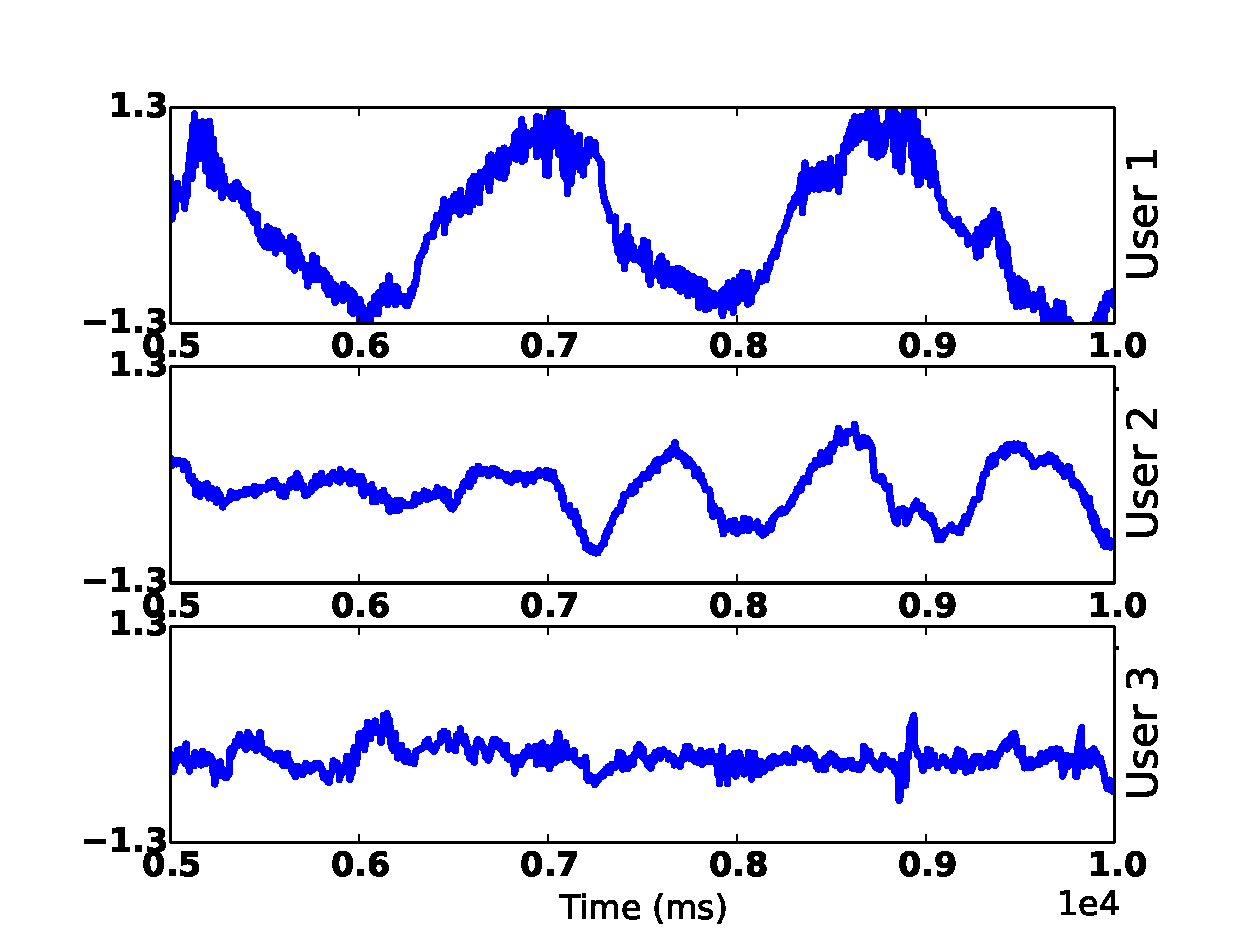
\includegraphics [width=.33\linewidth]{figure/raw_x.eps}&
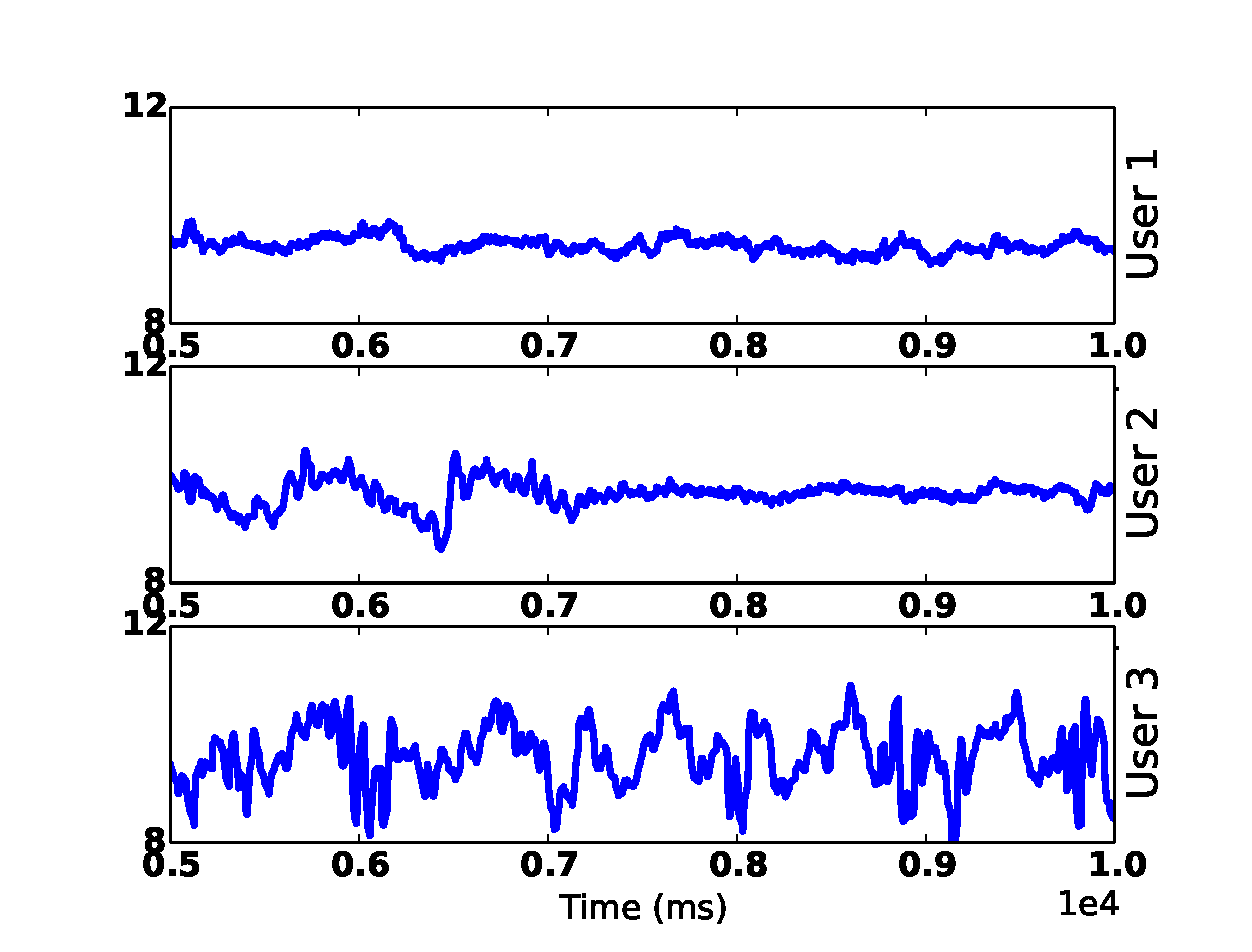
\includegraphics [width=.33\linewidth]{figure/raw_y.eps}&
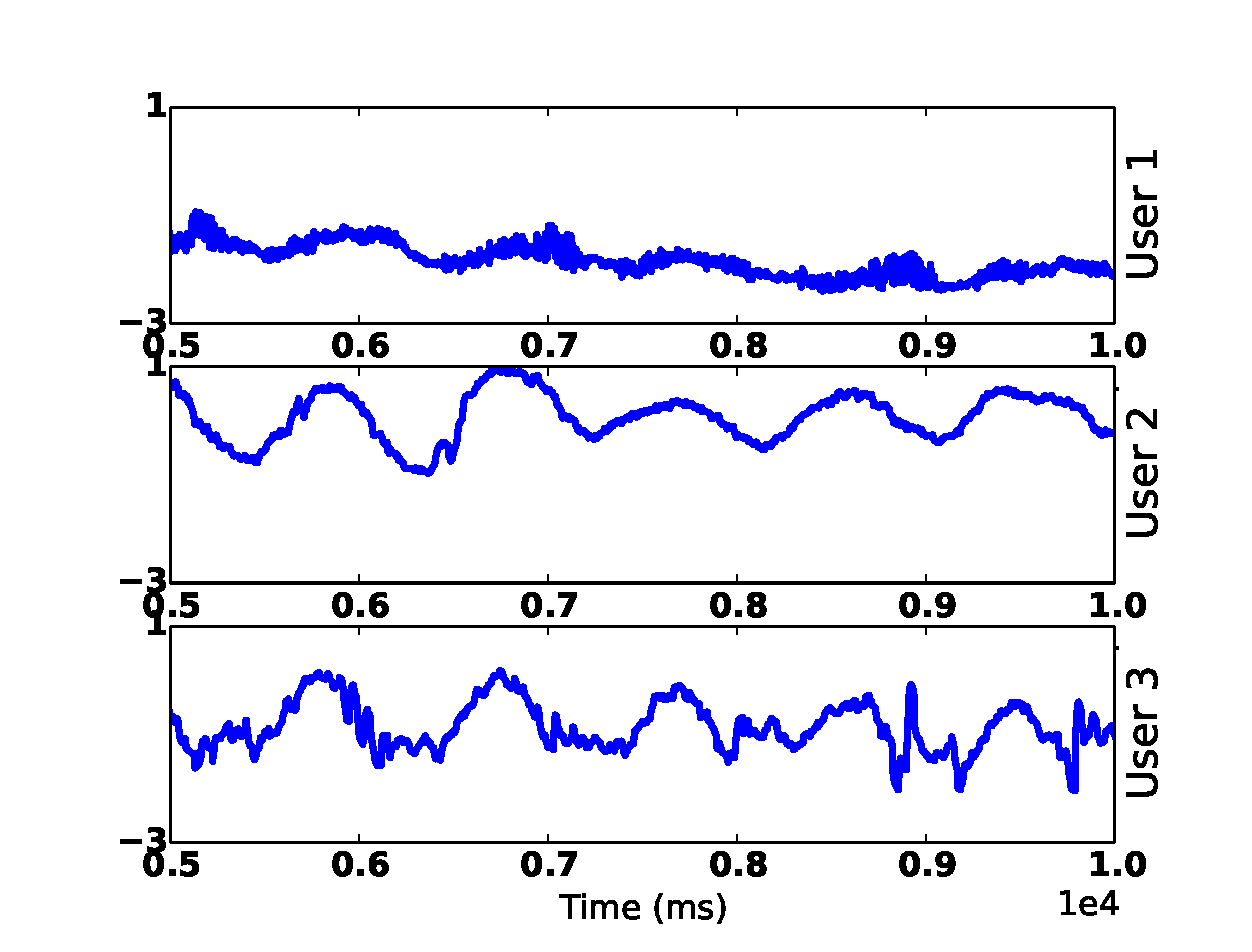
\includegraphics [width=.33\linewidth]{figure/raw_z.eps}\\
(a) X-Axis & (b) Y-Axis & (c) Z-Axis \\
\end{tabular}
%\begin{tabular}{cc}
%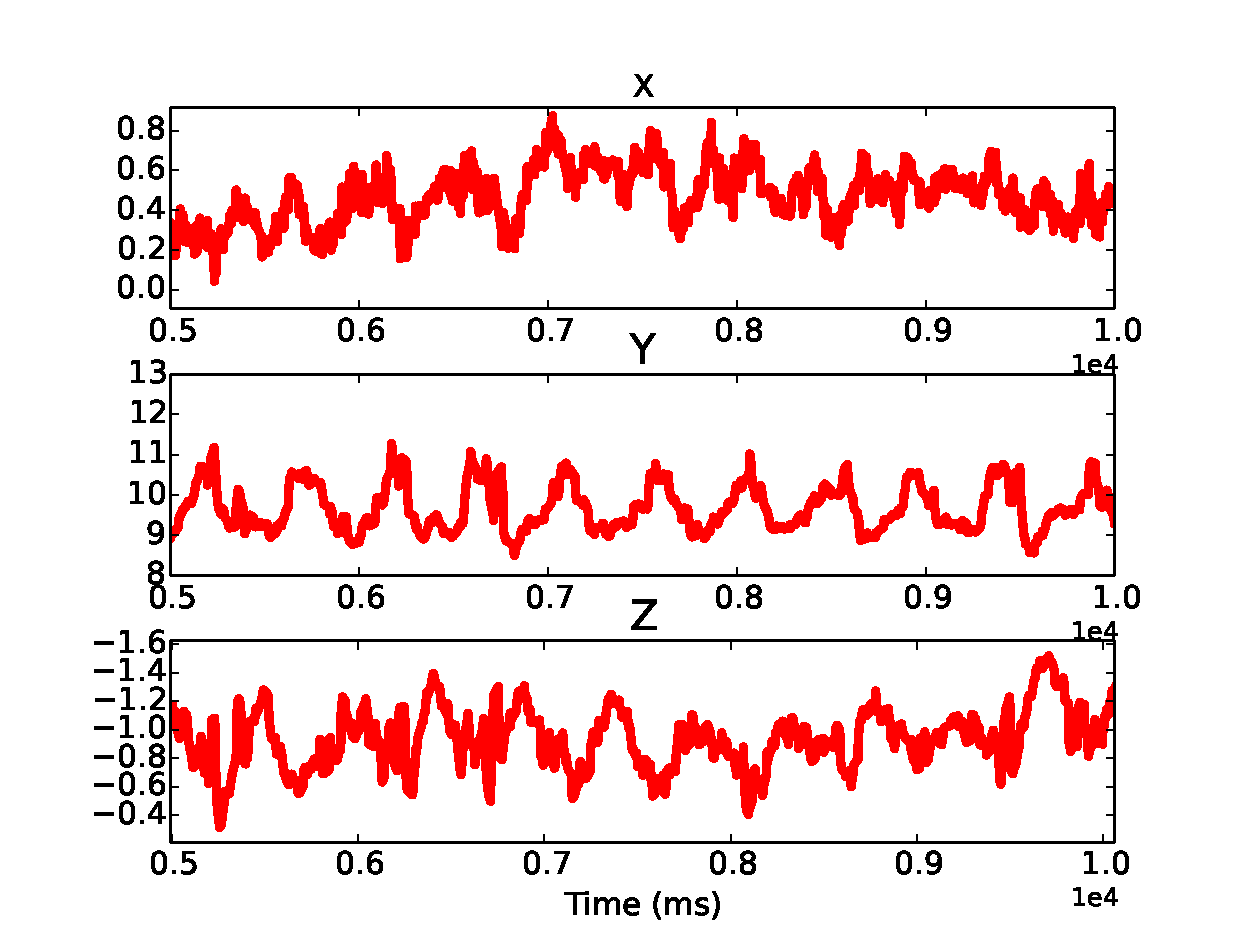
\includegraphics [width=.33\linewidth]{../fig/raw_sub4.eps}&
%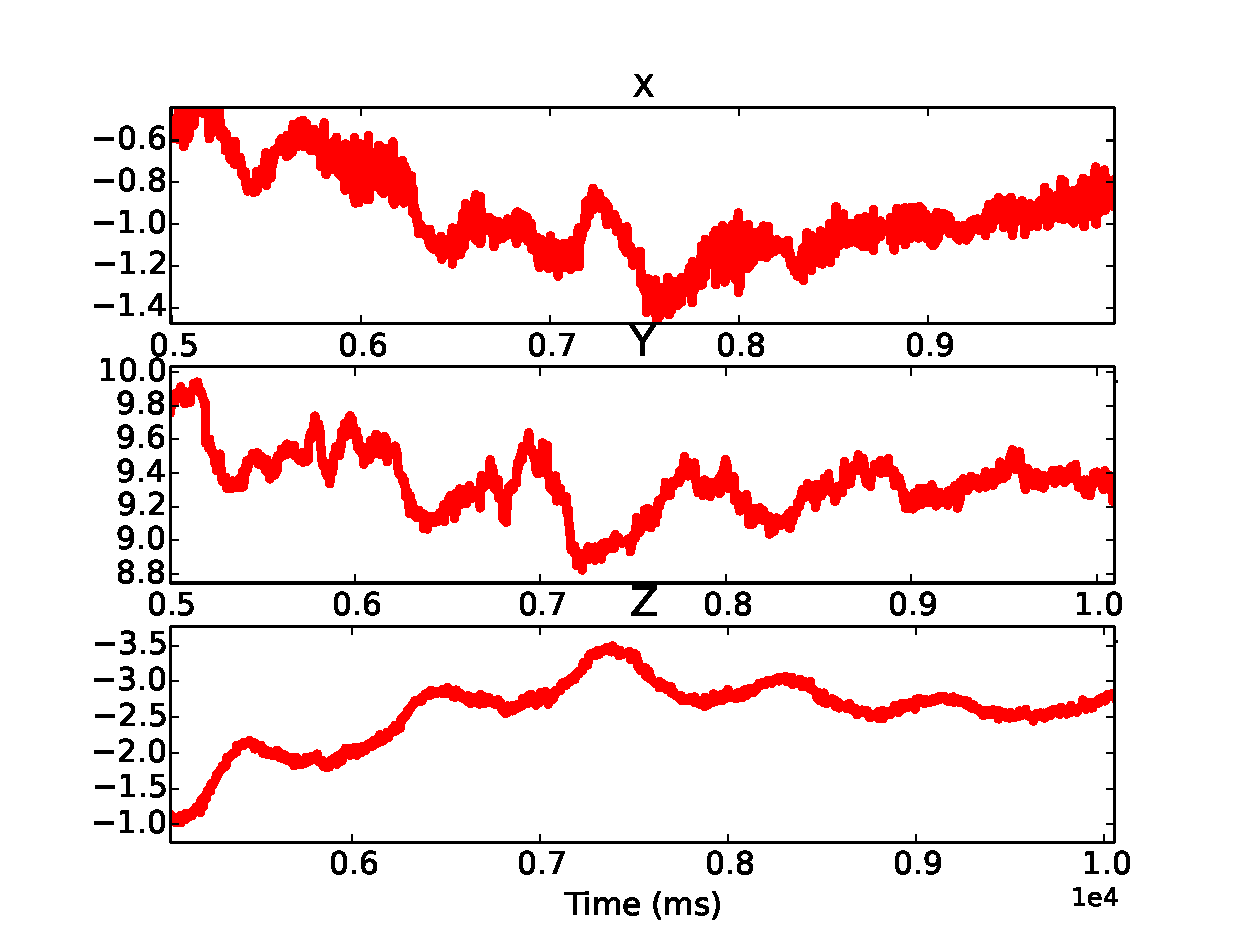
\includegraphics [width=.33\linewidth]{../fig/raw_sub5.eps}\\
%(d) User 4& (e) User 5 \\
%\end{tabular}
\end{center}
\caption{\label{fig:raw} These plots show the raw accelerometer data in the
time domain for five different users when they move their head in response to
the same music track wearing the same Google glass. The plots
indicate that different users' head movement patterns appear distinctive from
each other. The three users wore a Google Glass (in turns) and listened to a
10 second audio snapshot of a pop song.}
\vspace{-2pt}
\end{figure*} 


Based on a preliminary analysis of the accelerometer signals from three Google Glass
users, we observed (see Figure~\ref{fig:raw} (a)-(c))
that these users {\em repeatedly} showed {\em distinctive} head-movement patterns
(that are differentiable even through simple signal processing techniques),
when listening to the same music beats.

%Motivated by this observation we hypothesize that head movements
%can be a good behavioral biometric characteristic to authenticate
%users to their smart glass.
%We next formally present the design of our system that
%utilizes head-movement patterns as behavioral biometric signature
%to authenticate smart glass users.




\section{Headbanger System Design}\label{sec:design}

\begin{figure}[t]
\centering
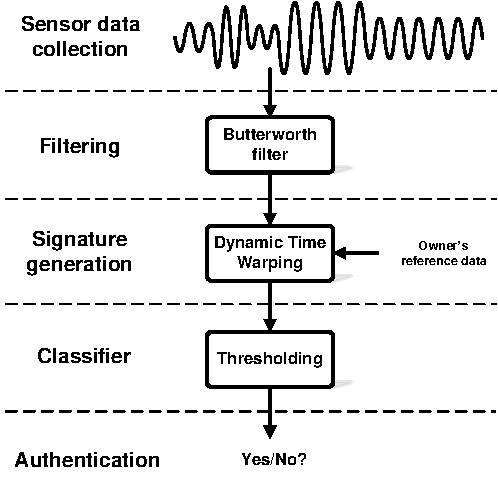
\includegraphics[width=.75\columnwidth]{fig/sysarch.eps}
\caption{\systemname~system design flow}
\label{fig:sysarch}
\end{figure}

\begin{figure*}[t]
\begin{center}
\begin{tabular}{ccc}
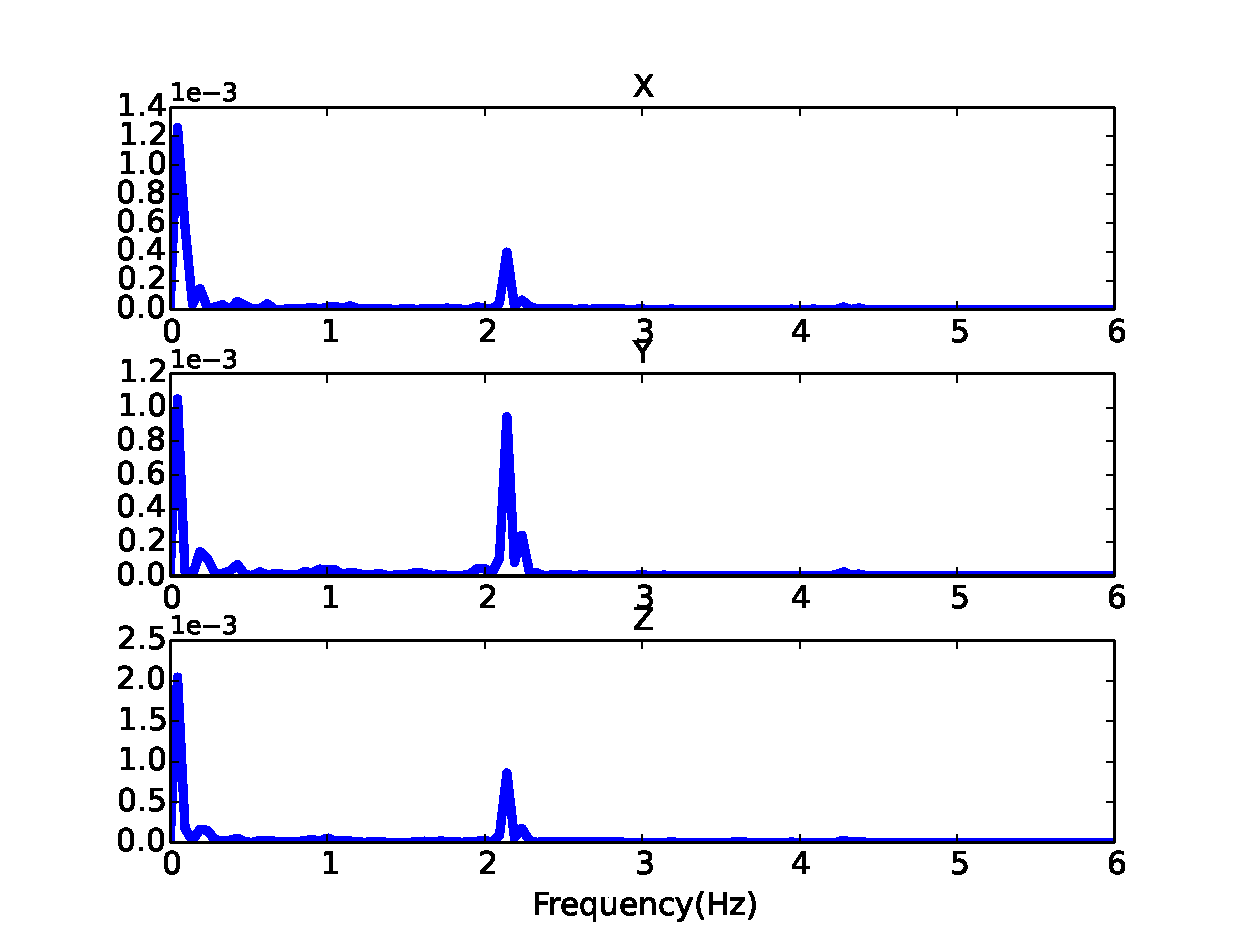
\includegraphics [width=.33\linewidth]{fig/freq_sub1}&
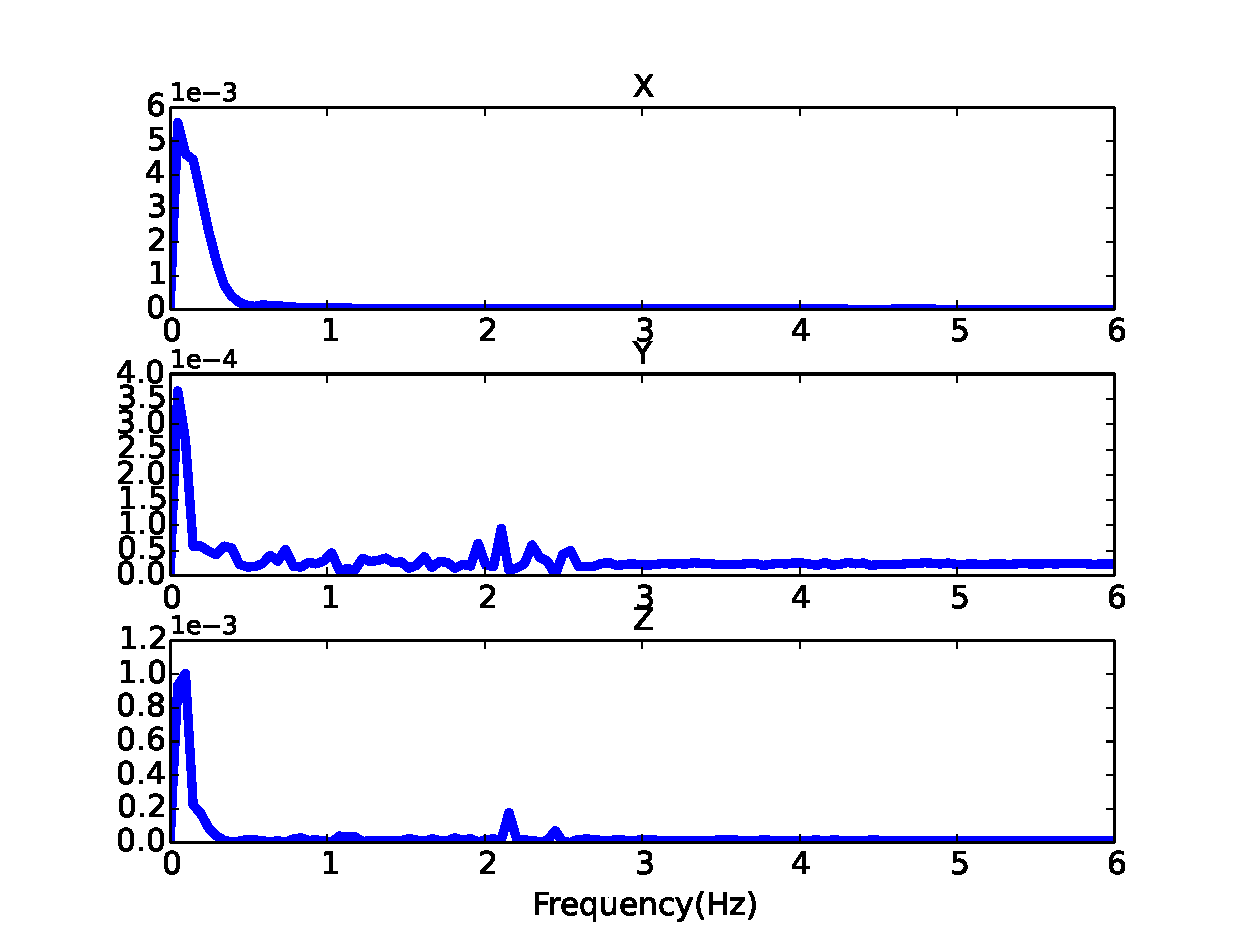
\includegraphics [width=.33\linewidth]{fig/freq_sub8}&
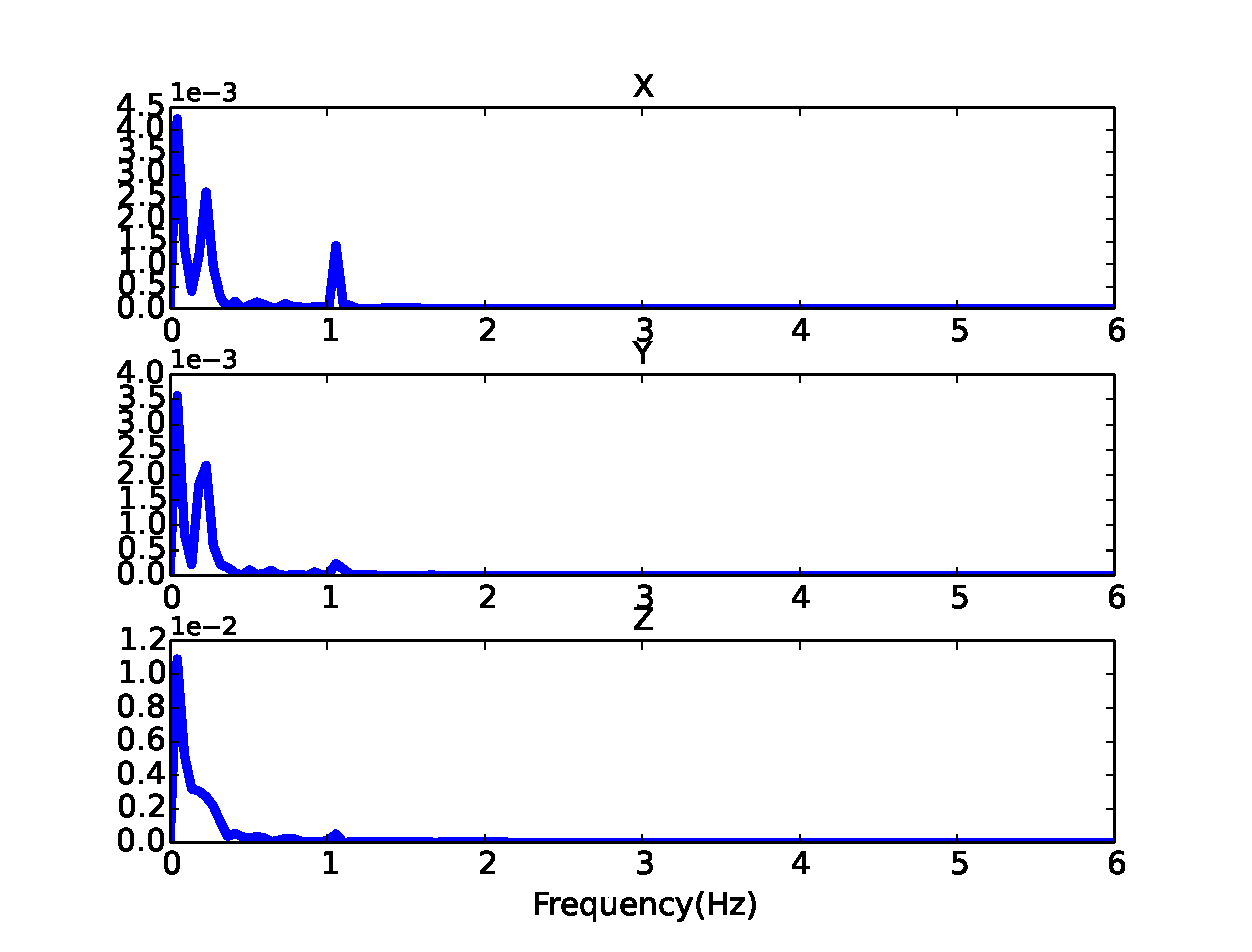
\includegraphics [width=.33\linewidth]{fig/freq_sub9}\\
(a) User 1& (b) User 2 & (c) User 3 \\
\end{tabular}

\begin{tabular}{cc}
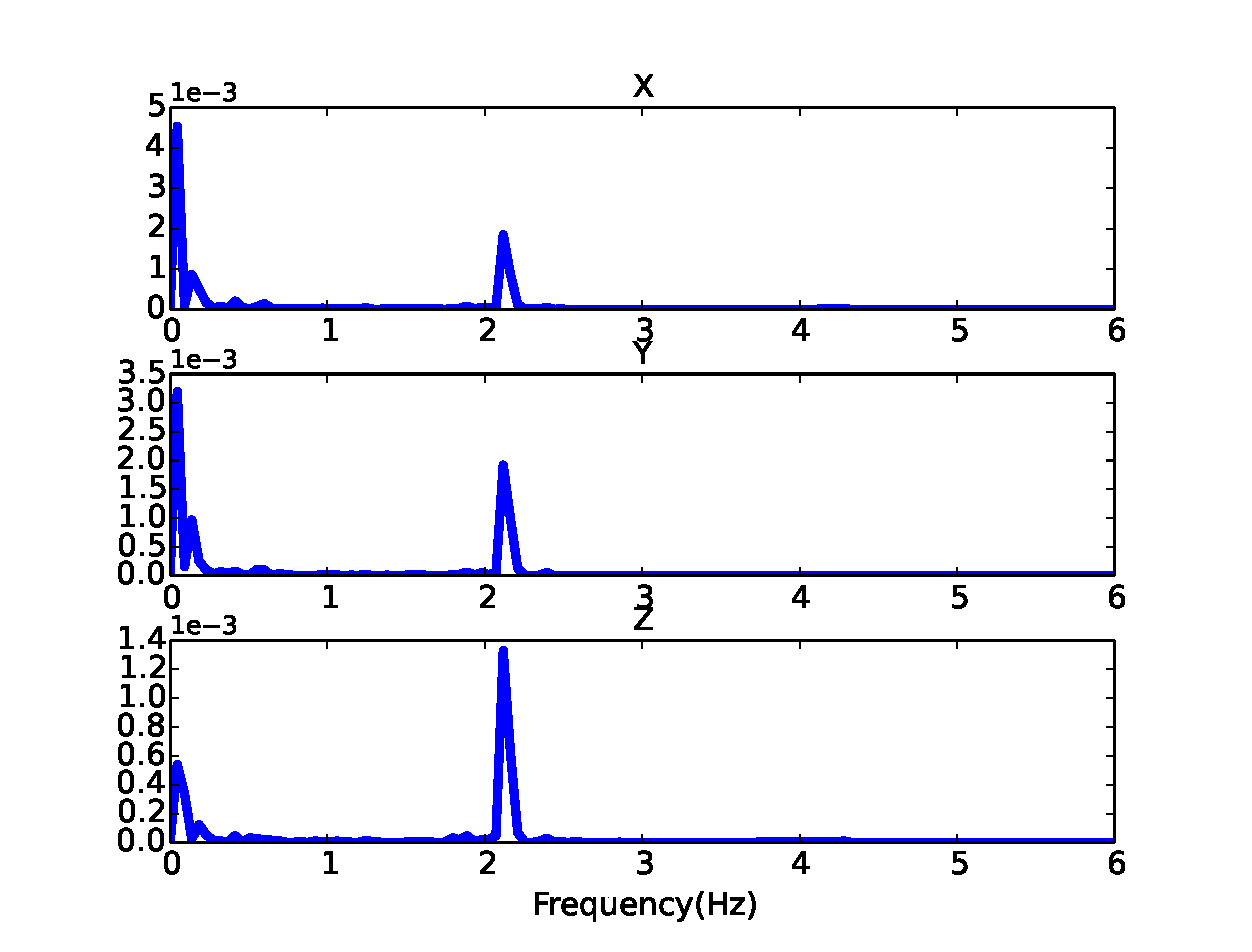
\includegraphics [width=.35\linewidth]{fig/freq_sub10}&
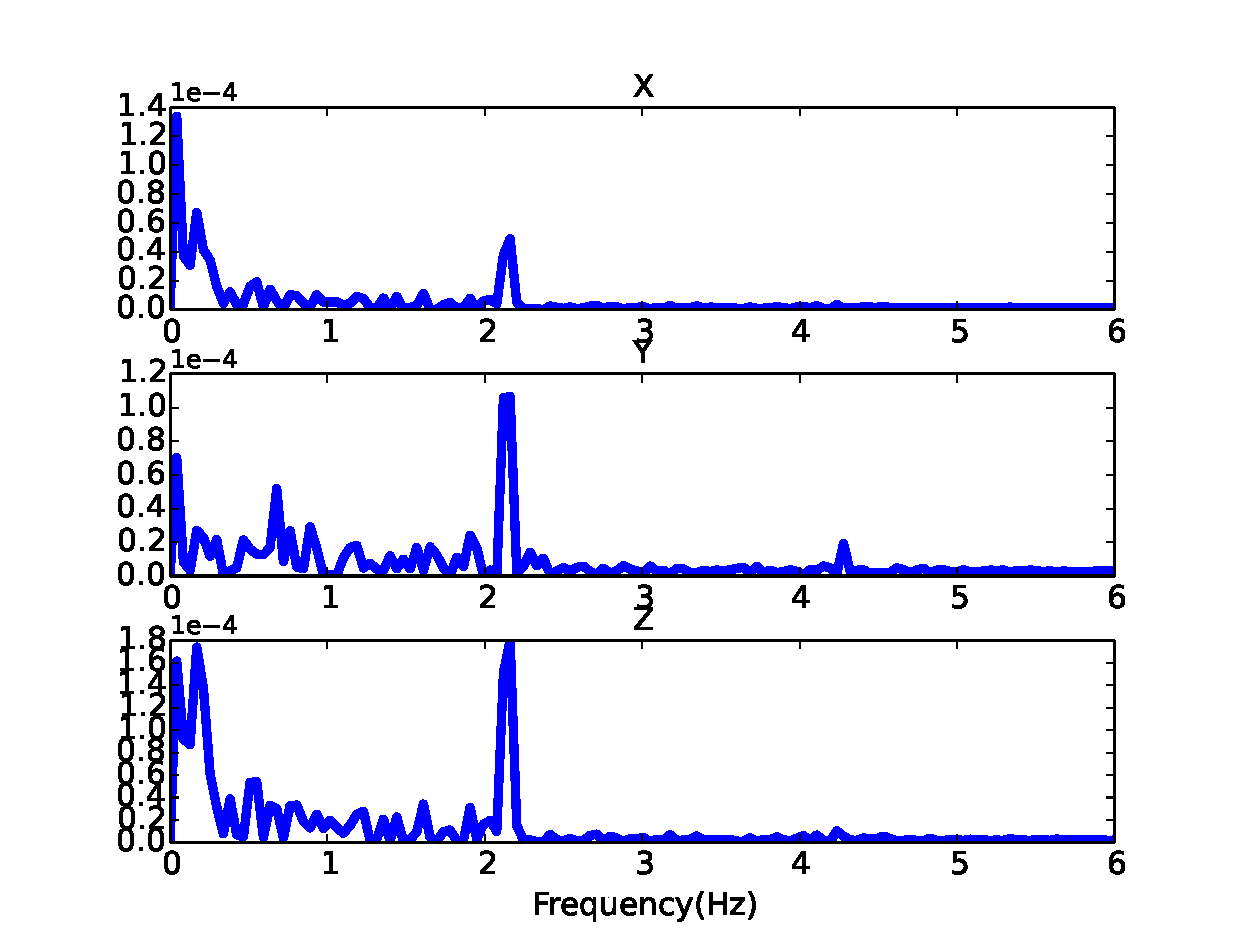
\includegraphics [width=.35\linewidth]{fig/freq_sub13}\\
(d) User 4& (e) User 5 \\
\end{tabular}
\end{center}
\caption{\label{fig:raw_freq} Accelerometer data from 5 people, in the frequency
domain. }
\end{figure*}

In this work, we design a system, \systemname, that will enable direct
authentication of users to their smart-glass device using
head-movements.
We envision that our proposed system will be used as an authentication
interface on the smart-glass wearable device.
The system will run as a service in the device upon power-up,
similar to the screen-lock in smartphones or the head-nod interface on Google
Glass~\cite{googleglass}. Upon usage, a short duration audio track
will be played on the device, and the user makes head-movements in
response to the audio. Our design is developed based on
the idea that humans respond to music naturally through head movements, and that such movements are more
significant and unique when the track contains fast beats and/or rhythm.
~\systemname~generates unique features from the head
movements of a user, and uses them as a biometric signature for
authenticating the right user to the device. The system will
grant access only when the head-movement signature
generated during the login attempt matches with the
original user's signature.

As illustrated in Figure~\ref{fig:sysarch}, the design of~\systemname involves the following key steps:
\begin{itemize}
\item {\em Sensor data collection}: ~\systemname~records the head-movements
in the form of raw accelerometer signals using the inbuilt accelerometer
sensor on the smart-glass device.
\item {\em Filtering}: The accelerometer signals are filtered by applying
a simple low-pass filter to remove records of extraneous motion.
\item {\em Signature generation}: The accelerometer signals are
processed through the dynamic-time warping (DTW) tool~\cite{dtw} to obtain a
DTW
feature that is treated as the unique signature for the user.
A user can generate different signatures for different audio tracks. A
training phase collects the set of signature for each user-audio pair.
\item {\em Classification}: The signatures are classified
to different users based on thresholding and machine learning strategies, and
labeled to the corresponding user.
\item {\em Authentication}: The head-movement signature generated
during system operation is compared with the original user-audio pair
signature, and the user is authenticated access if there is a plausible match.
\end{itemize}

%The original signature of the glass user is generated through a
%training phase that is executed when the glass is operated
%by the user for the very first time, and the training data gets
%updated upon each use of the device.
%As shown in Figure~\ref{fig:sysarch} shows the block diagram of
%~\systemname system design.
We will now discuss these design aspects in more detail.

\subsection{Sensor Data Collection}
%To facilitate natural head movement, we provide several
%short music tracks with easy-to-follow beats.

The sensor data collection step involves the user wearing
the head-worn device and making head-movements in response to
the music beats played on the device for $T$ seconds.
In this duration, the raw accelerometer
signals, from the inbuilt sensor, are collected at
a sampling rate of $r$ samples/sec; the default sampling rate on
Google Glass is 200Hz. Each accelerometer signal sample, referred
to as $ACC$ from here-on, is a collection of accelerometer readings on the
x,y, and z axis. The data collection unit stores each sample in a
matrix with dimensionality $3\times rT$ where each element corresponds
to one signal point of $ACC$. We retain the duration $T$ to be
in the order of few seconds, as frequency of human head
movements are, intuitively, typically in the order of few times per second
magnitude.
%The sensor data is accumulated in a $30r$ matrix, which we refer to as
%one $ACC$ sample.
%We hypothesize that
%head-movement can serve as a reliable behavioral biometric -- that is, $ACC$
%samples from the same user have smaller distances than samples from different
%users.

\begin{figure*}[t]
\begin{center}
\begin{tabular}{ccc}
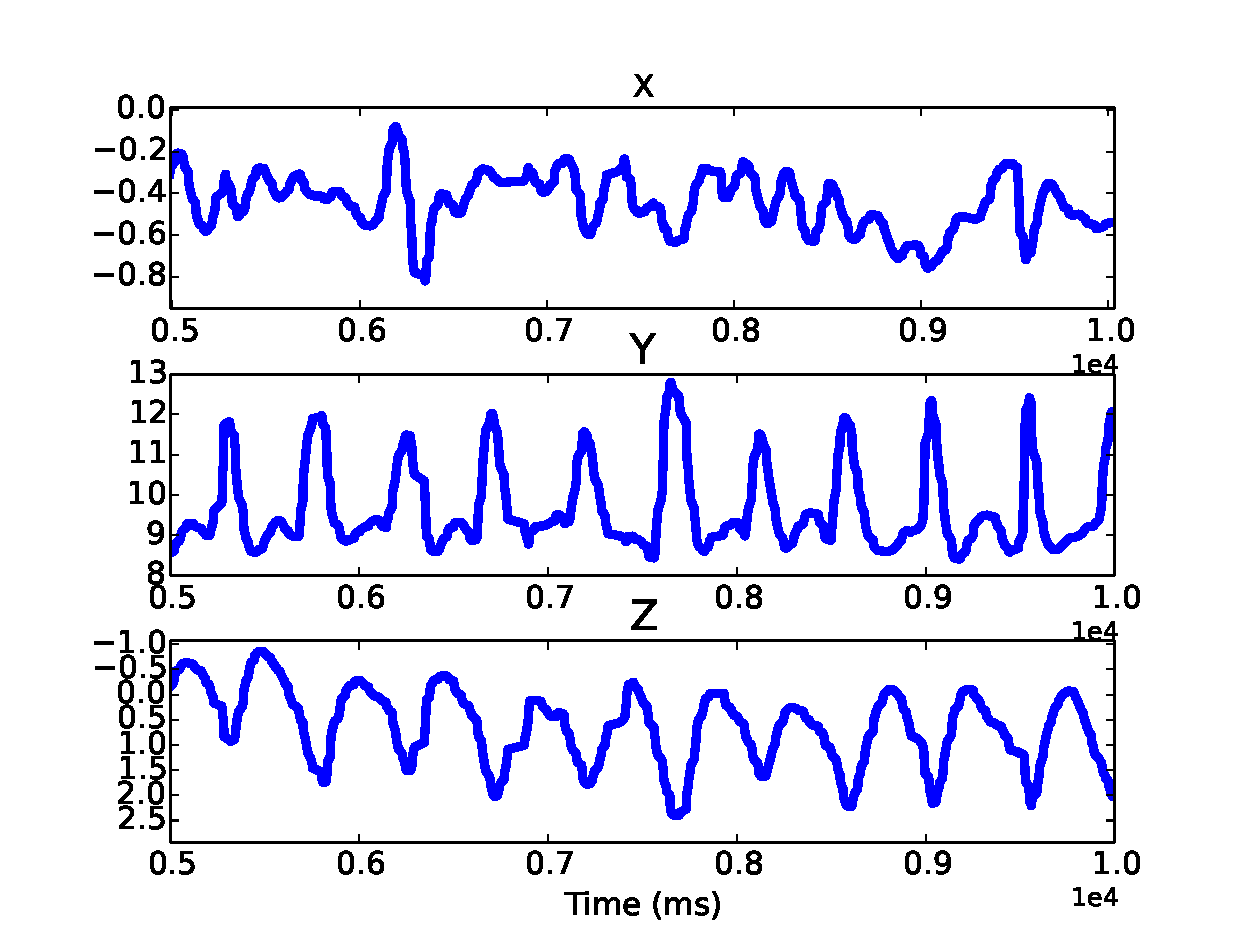
\includegraphics [width=.33\linewidth]{fig/filer_sub1.eps}&
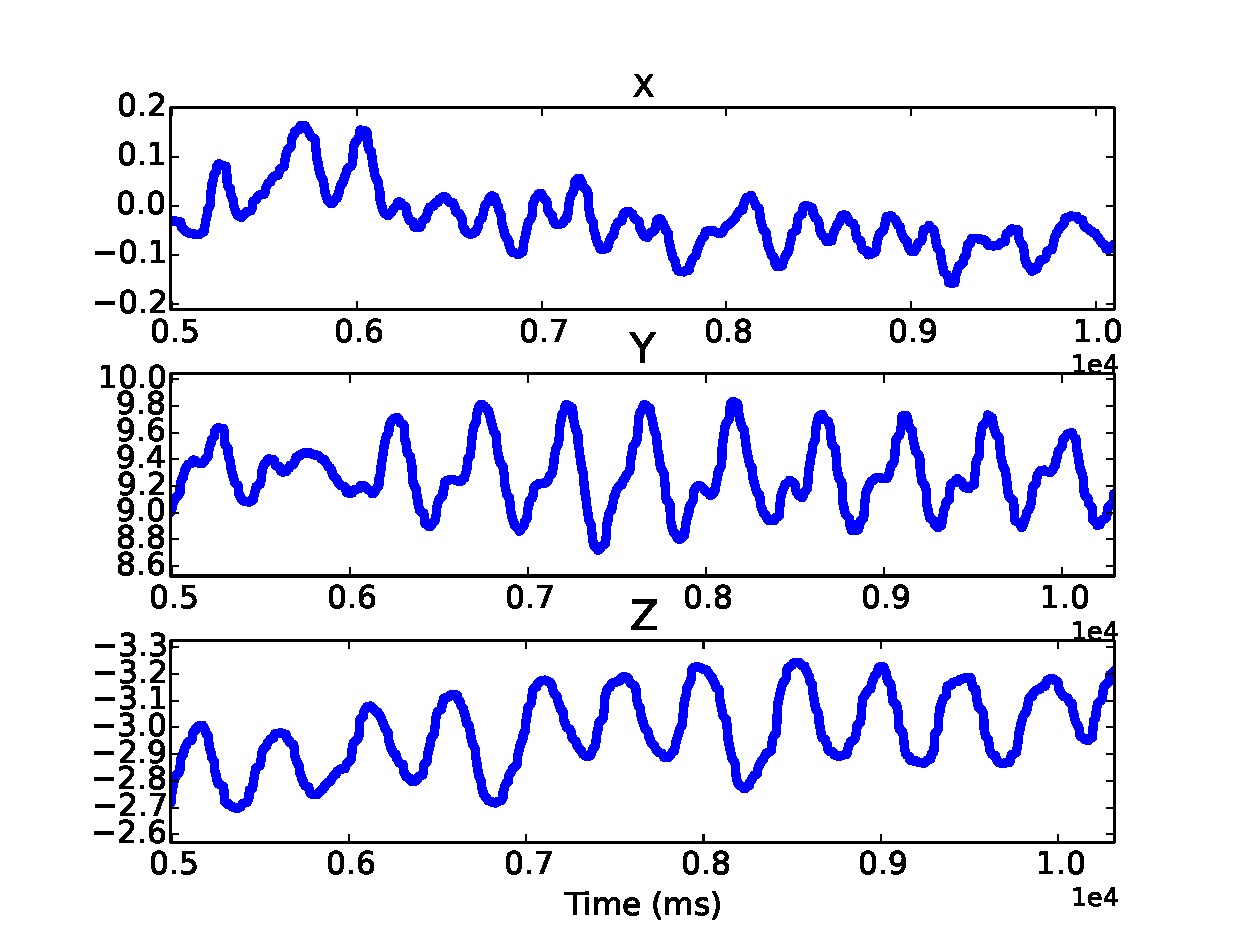
\includegraphics [width=.33\linewidth]{fig/filer_sub8.eps}&
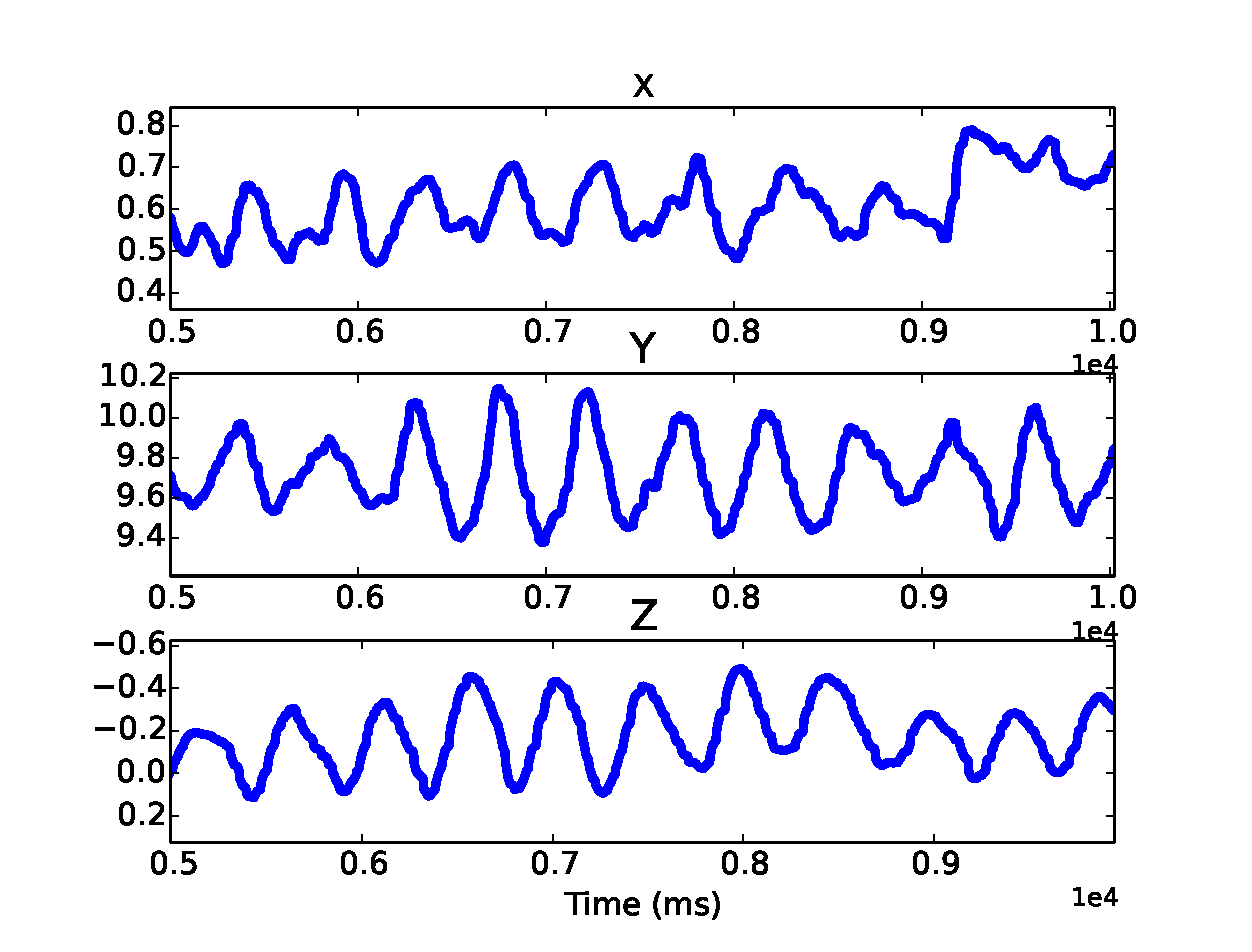
\includegraphics [width=.33\linewidth]{fig/filer_sub3.eps}\\
(a) User 1& (b) User 2 & (c) User 3 \\
\end{tabular}

\begin{tabular}{cc}
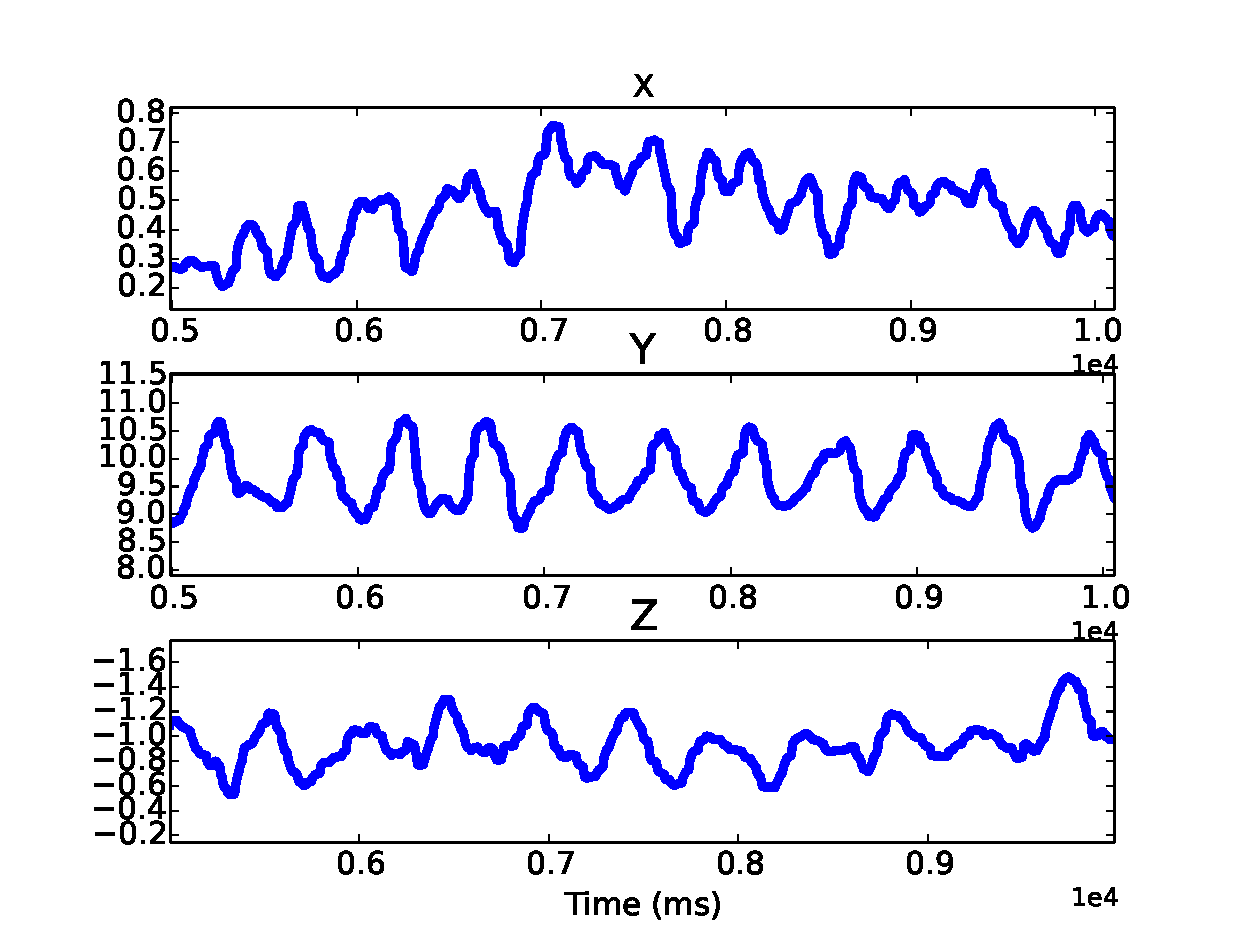
\includegraphics [width=.33\linewidth]{fig/filer_sub4.eps}&
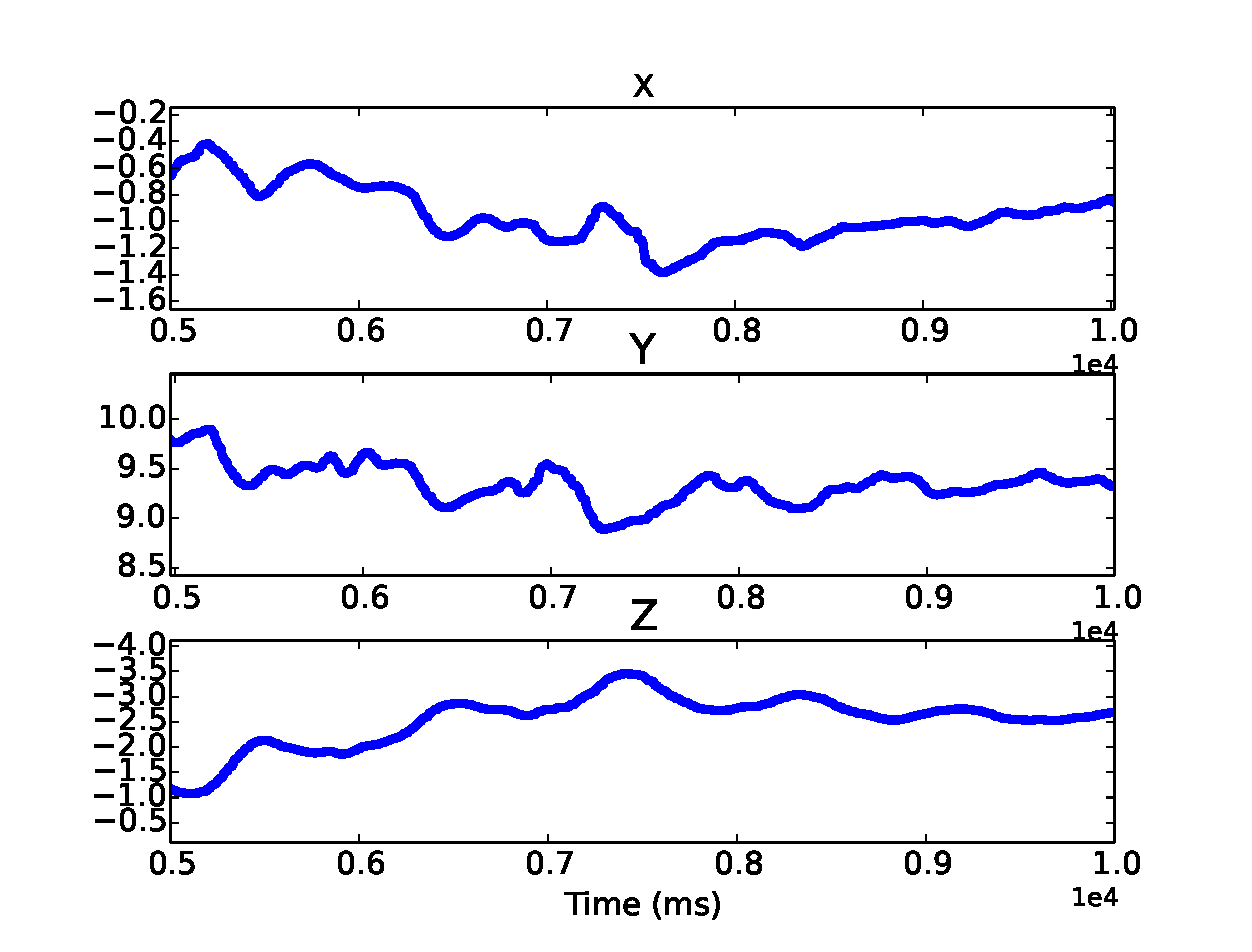
\includegraphics [width=.33\linewidth]{fig/filer_sub5.eps}\\
(d) User 4& (e) User 5 \\
\end{tabular}
\end{center}
\caption{Filtered accelerometer signals. Applied Butterworth
filter of order 2
and cut-off frequency 10Hz.\label{fig:filteredacc}}
\end{figure*}


\subsection{Filtering}

The $ACC$ samples are cleaned-up from noise (accelerometer
readings due to spurious movements such as vibrations) through
a filtering stage.
The filtering ensures that the head-movement signature
generated from the accelerometer readings encompasses
only head movements, and not any spurious signals caused due to
vibration or shaking. From the frequency
spectrum of each ACC sample, as shown in Figure~\ref{fig:raw_freq} for five users,
we can observe that the spectrum is significantly
concentrated within 5Hz.
We note that music tracks with high tempo, or fast beats, typically contain
beats in the order of the order of hundred beats per minute.
In particular, the high tempo music used in our experimentation was defined to
have 94 beats per minute~\cite{beats}.
We infer that the head-movement, in response
to the beats, will be of the same order. Hence, we hypothesize that
the signal spectrum in [0,5] Hz range encompass
human head movements; where 0 Hz can indicate that the head is
steady still, and 5 Hz can correspond to a vigorous head-shake.
We filter $ACC$ samples using a low-pass digital Butterworth
filter~\cite{challis1983design}. We set a relaxed cut-off frequency of 10Hz.
Even with the relaxed cut-off, the filtering results in
clean accelerometer samples with head-movement patterns
that are prominent and detectable. Figures~\ref{fig:filteredacc} (a)-(e) show the filtered results of the raw $ACC$ samples shown in Figure~\ref{fig:raw}; clearly, the filtered results are much more suitable for subsequent processing.

%\begin{figure}[t]
%\centering
%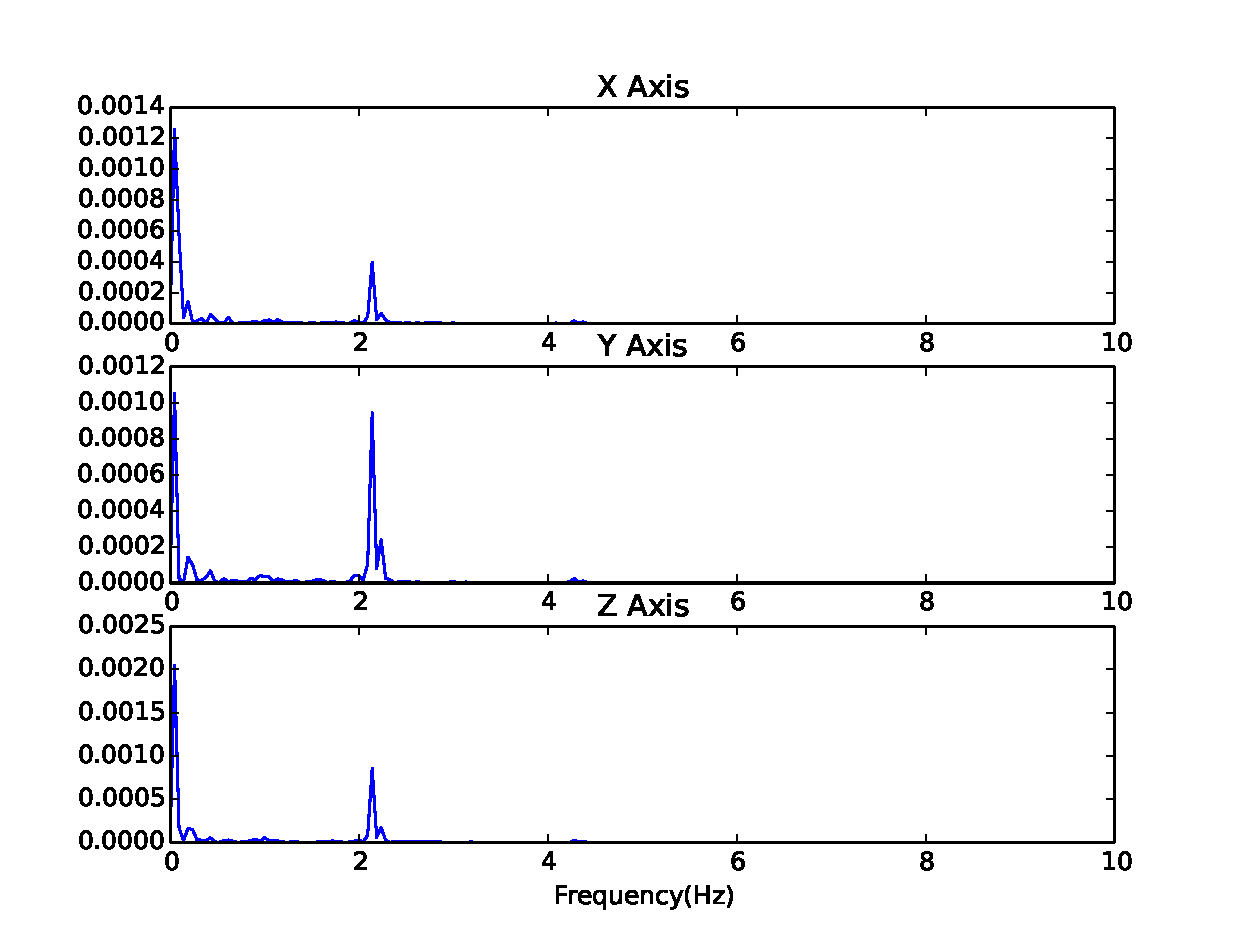
\includegraphics [width=.95\linewidth]{fig/freq_resp.eps}
%\caption{\label{fig:freq_resp}Fiver users' $ACC$ samples in frequency domain.}
%\end{figure}

\subsection{Signature generation}
%\subsection{Quantifying Sample Similarity}

We generate a signature from the accelerometer signals using the
dynamic-time warping (DTW) tool. DTW is generally used
as a similarity matching tool for time-domain analysis of
temporally varying signals.
DTW compares a temporal signal with a reference signal over a certain
time-window and yields a distance measure as the score. A low score (distance)
implies that the test signal is in close match with the reference.
We use the DTW principle to generate a signature for the head-movements
from the accelerometer signal.
We observed from our initial experiments that, users often
start head movement at a different angle,
but exhibit a consistent, and often periodic, patterns over time.
%We empirically observed that the accelerometer signal patterns
%are consistent after the first 1sec duration of head-movements.
Treating the $ACC$ sample set from the first trial as a reference, and we
apply the DTW algorithm on the successive $ACC$ sample set to obtain a
distance score vector, $\hat{d} = (d_x, d_y, d_z)$; the three elements in
$\hat{d}$ denote the DTW distance score in the $x, y, z$ axes, respectively.
By computing the mean of the distance scores obtained for each $ACC$
pair we generate the mean-value DTW distance, which is treated as the
head-movement signature for that particular user and audio
combination.
For evaluation purposes, we conduct an elaborate training phase where
$N$ trials of head-movement exercise are done, to obtain $N-1$ distance
vectors. In real usage of the application, the user would conduct only
two trials of $T$ duration each where trial 1 is treated as reference.
In this way, the training can be done in-situ. The training data-set is
updated upon each usage of the authentication interface.
%Small distance values DTW is expected to return relatively small distance
%values for samples from the same user, while returning large distance values
%for samples from different users (that have different movement patterns).
%Here, $S1$ is the reference

\iffalse
Next we investigate how we can accurately quantify the similarity level
between two $ACC$ samples, whose results will be used to classify the users.
After testing various methods,
We decide to adopt the Dynamic Time Warping (DTW) algorithm that is
often used to measure similarity between two waves based on temporal
stimulation.  Unlike many other algorithms, DTW measures the similarity
between two signals that are similar but with phase difference, which is well
suited for our study. In our study, users often start head movement at a
different angle, but exhibit similar, often periodic, pattern for a similar
amount of time. Applying the DTW algorithm on two $ACC$ samples $S1, S2$, we
get a vector $(d_x, d_y, d_z)$ denoting the distance in the $x, y, z$ axes
respectively. DTW is expected to return relatively small distance values for
samples from the same user, while returning large distance values for samples
from different users (that have different movement patterns).

YZ: Sugang, we need some detailed equations or algorithms here.
\fi

\subsection{Classification}
%\subsection{Classifying Users}
The classification step labels a test sample based upon the pre-established training samples, or trained signatures.
%the trained data-set, DTW signatures (distance
%vector), for each user-audio pair to its corresponding user.
%The classification step essentially separates ambiguous and spoofed
%authentication signatures from the original and generates a database
%of signatures for each user-device-audio pair. We will refer to this database
%as {\em trained signatures} for the rest of the paper.
%
In this work, we consider two classification mechanisms:
\begin{itemize}
\item {\em Supervised learning (SVM)}, which generates the trained signatures
for each user based on a training set that includes the user's original
signature as well as a number of other false signatures, that do not
correspond to the user.
\item {\em Adaptive thresholding}, which generates the trained signatures for
each user based on the signatures generated from a select set of trials of the
same user.

\end{itemize}

We will now discuss these two methods in more detail.

\subsubsection{SVM-Based Classification}
The SVM based classification goes through the following steps:
\begin{enumerate}
\item Construct the training set by including both ``true'' samples,
corresponding to the device owner, and ``false'' samples, corresponding to the
signatures from random users.
\item Calculate the DTW vectors between any two true samples (with the
resulting DTW vectors referred to as $DTW_{T\rightarrow T}$), as well as DTW
vectors between any true sample and false sample (with the resulting DTW
vectors referred to as $DTW_{T\rightarrow F}$).
\item Given a test sample $S$, calculate the
DTW vectors between $S$ and any true sample (with the resulting vectors
referred to as $DTW_{S\rightarrow T}$) as well as DTW vectors between $S$ and
false samples (with the resulting vectors referred to as $DTW_{S\rightarrow
F}$).
\item Input both, training DTW vectors (i.e., $DTW_{T\rightarrow T}$ \&
$DTW_{T\rightarrow F}$) and test DTW vectors (i.e., $DTW_{S\rightarrow T}$
\& $DTW_{S\rightarrow F}$) to a binary SVM classifier that labels each
signature with a $1$ or $0$ along with an identity corresponding to the
user-audio pair; a $1$ meaning the signature belongs to the right owner and
$0$ that it does not.
\end{enumerate}

{\bf Optimized SVM.} In order to minimize the computing overhead in the above
process and make it suitable for running on a smart-glass, we conduct the SVM
classification in an optimized fashion:
instead of looking at every single training sample from a user, we choose a
small set of representative samples and use them for classification.
Here, we define a user's representative samples as those that
are the most similar to samples from other trials (of the same user). Let us suppose a user's
entire training set has $N$ samples (from $N$ trials). For every sample, we
compute its distance to each of the $N-1$ samples using DTW. Then we choose
the $K$ samples that have the lowest $K$ average distance to the rest of the
training set. By setting an appropriate threshold $K$, we find the
representative samples from the training set. We refer to these $K$ samples as
top $K$ samples of the user. If we choose a small $K$ value, say 3 as opposed
to 20, the computing overhead can be significantly reduced. We conduct this
optimization strategy keeping in mind the increasing latency of SVMs with
training set size. We note to the reader that such an optimization is
only effective when the unoptimized training data-set size is sufficiently
large. %However, such a training data-set collection is a one-time procedure,
%while the top $K$ representative set is updated upon each login attempt of the
%user.
%For example, in our experiments, we use a unoptimized training set of
%size 10. In reality, however, we do not expect the user to generate
%signatures
%from 10 trials. Instead, we propose that the signatures
Eqn.~\ref{eq:top1} shows how we calculate the top 1 sample from $N$ samples
from a user.

\begin{eqnarray}
DTW_\mu & = &\frac{\sum_{i\neq{n}}DTW_i(n)}{N}\nonumber\\
DTW_{min} & = &min\{DTW_{\mu 1},...,DTW_{\mu N}\}
\label{eq:top1}
\end{eqnarray}

%In the testing phase, given a testing sample, we calculate its distance to each training set's top $K$ samples. Suppose we have $K$ true training samples, and $fK$ false training sets ($f$ is the number of false training sets), then we will have $(f+1)K$ distance values for the testing sample. We then input these distance values to the SVM classifier which will return the classification result -- $1$ means the user is classified as the owner while $o$ means the user is not classified as the owner.


\subsubsection{Adaptive thresholding-Based Classification}

Through empirical trials we observed that the SVM classification may not be very
robust against false training signatures that come very close to the true
samples. While finding optimal binary SVM classifier parameters or using a
multi-class SVM~\cite{weston1999support} are probable solutions, we felt that these
approaches will add significant overheads to the already complex SVM.
As an alternative, we developed a simple yet effective classification scheme
based on adaptive thresholds.
We highlight the aspects of the adaptive thresholding procedure as follows:
\begin{enumerate}
\item Given $N$ true training samples, identify the top $K$ samples
(representative set), and calculate their DTW vectors to the rest of the
samples in the training set to obtain $(N-1)K$ distance vectors. Call this
resultant vector as top-$K$ distance vector.
\item Compute the 3 element (x,y,z axis) mean $\mu$ vector and standard
deviation $\sigma$ vector of the top-$K$ distance vector. Define the
``true'' range as $[\mu-m\sigma, \mu+m\sigma]$, where $m$ is a design
parameter that will be fixed by the designer. The samples outside this
range are labeled as ``false''.
We refer to this range $[\mu-m\sigma, \mu+m\sigma]$ as the threshold in our
classifier design.
%\item Steps (1) to (3) are repeated when a new sample set is added to the
%training database resulting in an updated threshold. This way, the thresholding
%based classification is adaptive to the user trials. As we will show in our
%evaluations, the thresholding approach is more robust than the SVM approach,
%through both yield reasonable authentication accuracy.
\end{enumerate}

\subsection{Authentication}

The authentication step results in a binary output that corresponds to
either allowing or disallowing the user to unlock the device.
In this paper, we make two reasonable assumptions pertaining to authentication
on the smart-glass device: (i) homogeneity of
accelerometer sensors for all smart-glasses (from a particular vendor), and (ii)
that the device is registered to the user with an associated PIN or passcode,
and that the head-movement signature is used for secondary verification.
Upon entry of the correct password, the device verifies the identity
of the user based on the head-movement signature.

In the head-movement authentication phase, given a test sample, we classify the sample as true (1) or false
(0) based on one of the two classifiers discussed above. If the result is true, the user is accepted; otherwise
the user is rejected.

%The authentication mechanism for each of the two classification strategies are
%as follows:

%{\bf SVM.} Given a test sample, classify the sample as true (1) or false
%(0) based on the SVM classifier. %If the result is true, compute the euclidean
%distance between the each of the top $K$ true signatures and the classified
%test signature. If the euclidean distance is below a pre-set threshold
%(obtained empirically from training phase)


%{\bf Adaptive thresholding.} Given a testing sample, calculate the
%DTW distance between the testing sample and the top $K$ representative
%samples. If the resulting distance mean falls within threshold range, then the
%result is ALLOW USER; otherwise, the user is rejected.

%\input{recognizing}
\section{Evaluating Headbanger System}\label{sec:results}

We conducted extensive evaluation of the Headbanger system. In particular, our evaluation focused on showing that a user's body movement pattern can be used to establish the user's identify. We first show that even a simple movement pattern is hard to imitate by others (i.e., being distinctive), and next show that people can easily repeat their own patterns (i.e., being repeatable). To conduct the evaluation, we prototyped the Headbanger system using the Google Glass, but our system can be easily implemented on other platforms.

\begin{figure}[t]
\centering
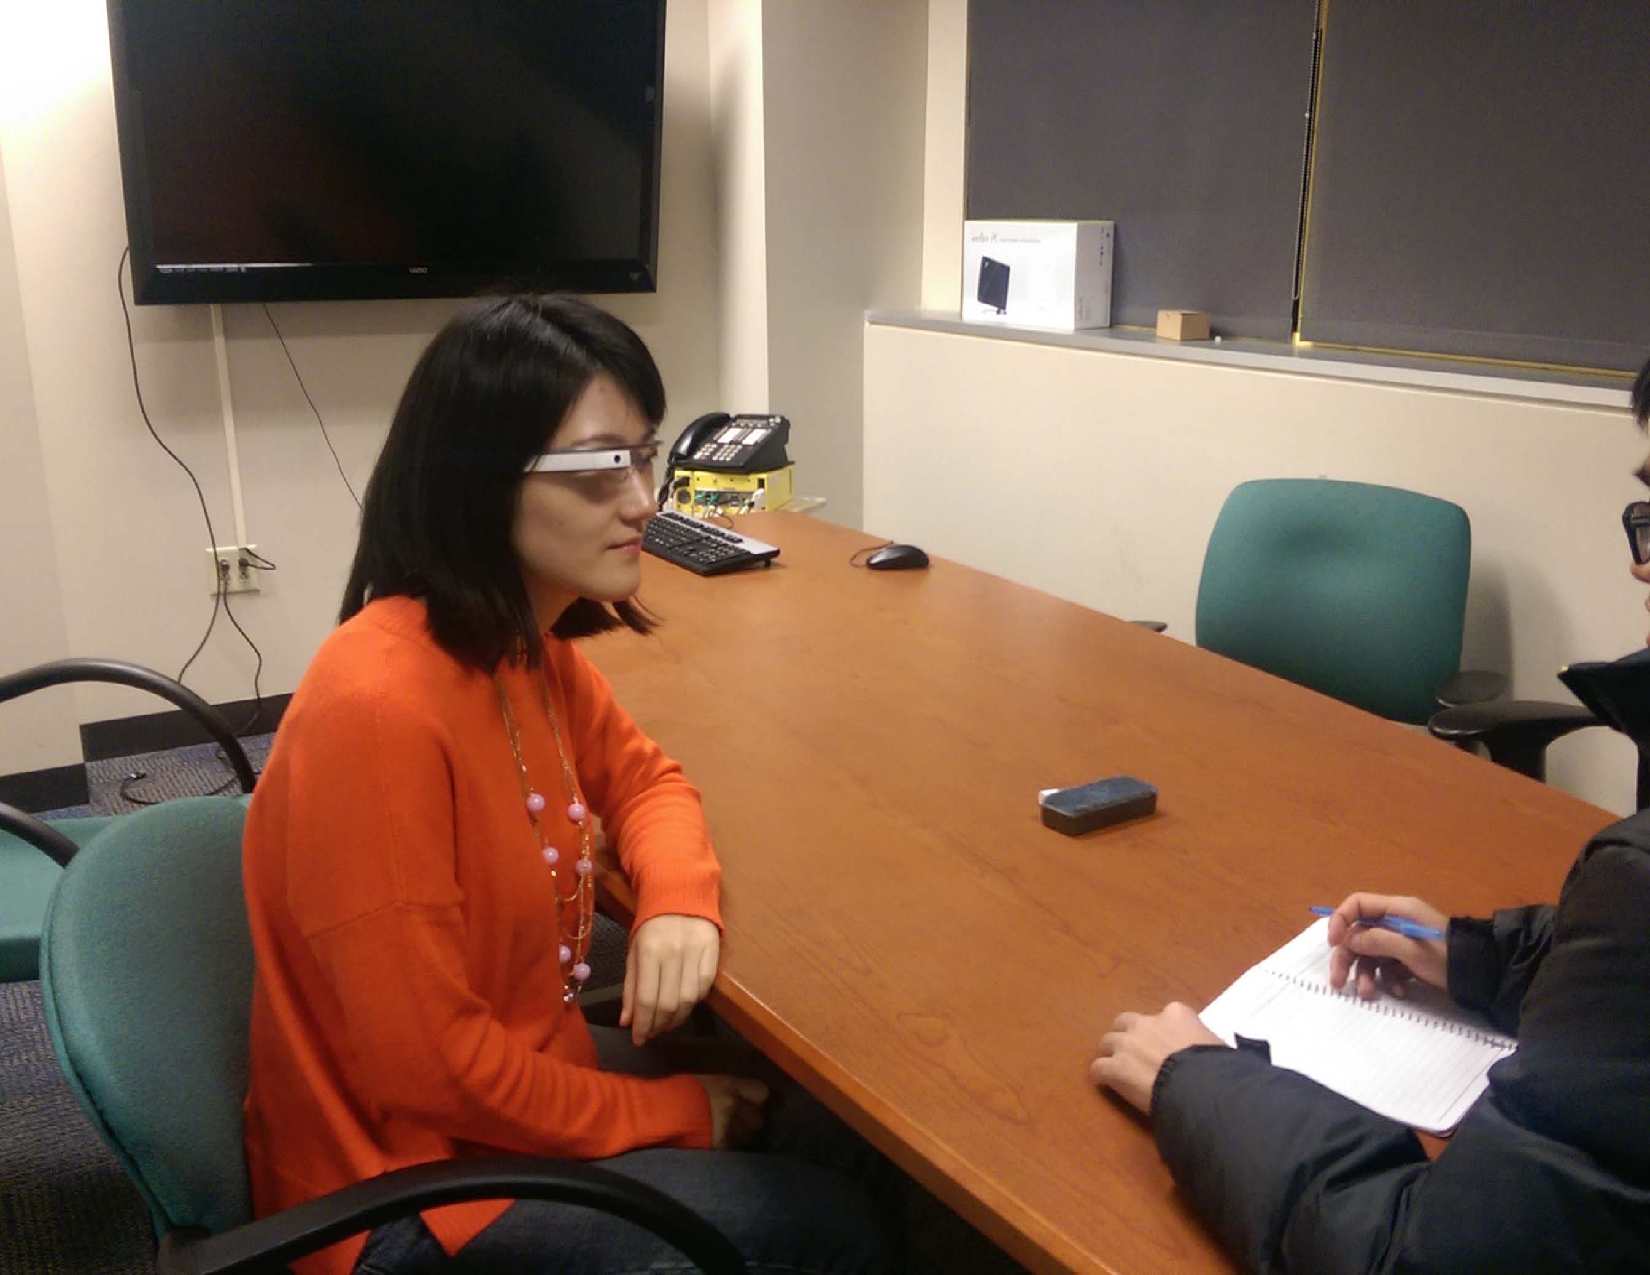
\includegraphics [width=.75\columnwidth]{fig/exp.pdf}
\caption{Our team member was collecting data with one of the participants. \label{fig:exp}}
\end{figure}


\subsection{Dataset}

We collected head-movement $ACC$ samples from 24 subjects. We informed the participants of the risks involved in wearing Google Glass and collecting head-movement data (e.g., feeling dizzy after head-movement for a period of time, not being able to see clearly if near-sighted, etc.). If they agreed to participate, we asked each subject to report their age and gender. We asked the subjects to wear the Google Glass and make head-movements while listening to the music track. Meanwhile, we recorded the raw accelerometer data.  Each recording session was 10 seconds long, and we sat through each session with the subject to help him/her use the system properly, as shown in Figure~\ref{fig:exp}. After every 5 recording sessions, we asked the subject to take a break to relax their muscle and regain energy. Both our system design and our data collection protocol were approved by our Institutional Review Board. The subjects, 12 females and 9 males, had an average age of 26 years.

\subsection{Even Simple Body Movement is Hard to Imitate}\label{sec:experimenr2}
In the first set of experiments, we show that even simple body movement is very hard to imitate by others, and thus body movement is rather distinctive among different people.

\subsubsection{Experimental Setup}
One of the simplest body movement patterns that can be easily captured by built-in sensors is nodding, which we employed in this set of experiments. The audio file we used in the experiments can be downloaded at \emph{http://www.winlab.ru\\
tgers.edu/~sugangli/somebody.midi}.

Each $ACC$ sample was collected for the duration of 10 seconds. When calculating the classification results, we generated shorter samples of varying lengths (2 seconds, 3 seconds, 6 seconds, and 10 seconds) from the original 10-second samples. The sum of the sample duration and the subsequent processing latency thus determines the authentication response time of our system. Longer sample durations likely lead to more accurate classification results, but shorter sample durations may be preferred by users due to faster authentication responses.

In this set of experiments, we have one glass owner, who designed the nodding pattern,  and 15 imitators who imitated the movement. We collected 100 10-second $ACC$ samples from the owner, during the course of 60 days (from 10/1/2014 to 11/30/2014), ensuring the owner's sensor data includes sufficient variation that naturally occurs with time. We also made a great deal of effort to make sure the imitators accurately imitate the owner's movement -- the owner carefully explained his movement pattern to each imitator, and sat through each data collection session for all the 15 imitators to make sure their movement pattern looks the same to the owner's eye. For reach imitator, we collected 40 10-second $ACC$ samples.






\begin{table}[b]
\small
\begin{tabular}{|l||l|l|l||l|l|l|}\hline
& \multicolumn{3}{|c||}{2}& \multicolumn{3}{|c|}{3}\\\cline{2-7}
Sample duration (s)& FRR & FAR & BAC & FRR & FAR & BAC\\
&(\%) &(\%) &(\%) &(\%) &(\%) &(\%)\\\hline

SVM Top 1                 & 25.0 & 16.74 &79.12 & 15.0 & 14.05 & 85.47  \\\hline
SVM Top 3 Voting          & 14.84& 9.24 & 87.95 & 18.48 & 6.85 & 87.33  \\\hline\hline

& \multicolumn{3}{|c||}{6}& \multicolumn{3}{|c|}{10}\\\cline{2-7}
Sample duration (s)& FRR & FAR & BAC & FRR & FAR & BAC\\
&(\%) &(\%) &(\%) &(\%) &(\%) &(\%)\\\hline

SVM Top 1                   & 3.33& 6.66& 95.0  & 0.0& 9.62& 95.18 \\\hline
SVM Top 3 Voting            & 7.27& 6.17& 93.27 & 4.84& 6.17& 94.48 \\\hline

\end{tabular}
\caption{Average FAR, FRR, and BAC for SVM-based classification when we choose different 4 imitators in the training set (from the total 15 imitators). We have the results for different sample durations. In these results, we use the earliest 40 owner samples in the training set.\label{tab:kfoldfalse-svm}}
\end{table}

\iffalse
\begin{table}[b]
\small
\begin{tabular}{|l||l|l|l||l|l|l|}\hline
& \multicolumn{3}{|c||}{2}& \multicolumn{3}{|c|}{3}\\\cline{2-7}
Sample duration (s)& FRR & FAR & BAC & FRR & FAR & BAC\\
&(\%) &(\%) &(\%) &(\%) &(\%) &(\%)\\\hline

SVM Top 1                   & & &83.64 & & & 87.11  \\\hline
SVM Top 3 Voting            & & & 84.90 & & & 88.96 \\\hline\hline

& \multicolumn{3}{|c||}{6}& \multicolumn{3}{|c|}{10}\\\cline{2-7}
Sample duration (s)& FRR & FAR & BAC & FRR & FAR & BAC\\
&(\%) &(\%) &(\%) &(\%) &(\%) &(\%)\\\hline

SVM Top 1                   & & & 90.68 & & & 92.63 \\\hline
SVM Top 3 Voting            & & & 91.38 & & & 93.02 \\\hline

\end{tabular}
\caption{Average FAR, FRR, and BAC for SVM-based classification when we choose different 40 owner samples in the training set (from the total of 100 samples).  We have the results for different sample durations. In these results, we use the first four imitators in the training set.\label{tab:kfoldtrue-svm}}
\end{table}
\fi

\subsubsection{Classification Metrics}
In this study, we consider both SVM based classification and thresholding based classification. The classification process is different for these two approaches:

\begin{itemize}
\item \emph{SVM based classification.} For SVM based classification, we need to construct a training set that consists of both true training data (from the owner) and false training data (from the imitators). In total, we have 100 data samples from the owner and $15 \times 40$ samples from imitators, from which we include $S$ samples from the owner, and all the samples from $I$ imitators ( $I \times 40$ samples) in the training set. Therefore, we have $100-S$ owner samples, and $(15-I)\times 40$ imitator samples in the testing set.


\item \emph{Thresholding based classification.} For thresholding based classification, the training set only consists of data samples from the owner. Similar to the SVM case, we use $S$ samples from the owner as the training set, and all the other samples as the test data.
\end{itemize}

In our evaluation, the default value for $S$ is 40, and the default value for $I$ is 4. In the evaluation, we varied the value of $S$ and $I$ as well as the chosen training samples to ensure the robustness of our system~\footnote{In the interest of space, we didn't include the results with different I values in this paper.}.


For both SVM-based and thresholding-based classification approaches, we consider two testing methods. The first method involves comparing the test sample against the top 1 training sample from a user, which we refer to as \emph{Top 1} testing. The second method involves comparing the test sample against the top 3 training samples from a user and then determining the classification result by voting among these three results, which we refer to as \emph{Top 3 Voting} testing.

In this study, we consider classification metrics that are popular in biometric authentication, namely false acceptance rate $FAR$ (the percentage of false test samples that are mistakenly accepted) and false rejection rate $FRR$ (the percentage of true test samples that are mistakenly rejected). Usually, an overly strict classification system leads to high $FRR$, while an overly relaxed system leads to high $FAR$. We also consider balanced accuracy $$BAC = 1 - (FAR+FRR)/2,$$ which is a combined metric that measures both $FAR$ and $FRR$.



\subsubsection{SVM Classification Results}

As mentioned earlier, SVM classification requires training data from both the owner and imitators. In the results shown in Table~\ref{tab:kfoldfalse-svm}, we used the earliest 40 samples from the owner (out of 100 total owner samples), but varied the imitators that are included in the training set. Specifically, if we label the 15 imitators as $I_1, ..., I_{15}$, then we had the following 15 different combinations of imitators in the training set: $\{I_1, I_2, I_3, I_4\}$, $\{I_2, I_3, I_4, I_5\}$, $\dots$, $\{I_{15}, I_1, I_2, I_3\}$.  Table~\ref{tab:kfoldfalse-svm} shows the average FAR, FRR, and BAC values over these 15 combinations. By considering these different cases, we can eliminate the impact of having a specific imitator in the training data and the results are more representative. Here, we also vary the sample duration: 2, 3, 6, and 10 seconds.

From Table~\ref{tab:kfoldfalse-svm}, we have the following main observations:

\begin{enumerate}
\item \emph{Even simple nodding is not easy to imitate: nodding for 6 seconds can classify 95\% of the users.} As the sample duration increases from 2 seconds to 6 seconds, the classification accuracy improves significantly -- the BAC value changes from 79.12\% to 95\% for top 1 testing, and from 87.95\% to 93.27\% for top 3 voting. After the sample duration reaches 6 seconds, the improvement becomes less pronounced. This suggests that a sample duration of 6 seconds is sufficient to successfully classify 95\% of the users. We feel that moving our head gently along with music for 6 seconds is in general not a cumbersome process for most users. It further suggests that even simple nodding is hard to imitate by others, and thus head-movement has the potential to serve as a reliable biometric characteristic for smart wearable authentication.


\item \emph{For sample duration of 6 seconds, testing against 1 training sample is sufficient.} The results also show that, when the sample duration is short (e.g., 2 or 3 seconds), comparing the test sample against top 3 training samples leads to much better classification result. When the sample duration is reasonably long, say 6 seconds, comparing the test sample against the top 1 training sample leads to better results. This is advantageous because top 1 testing incurs much less processing and energy overhead, lending itself for execution on wearable devices.
\end{enumerate}


\begin{figure*}[t]
\centering
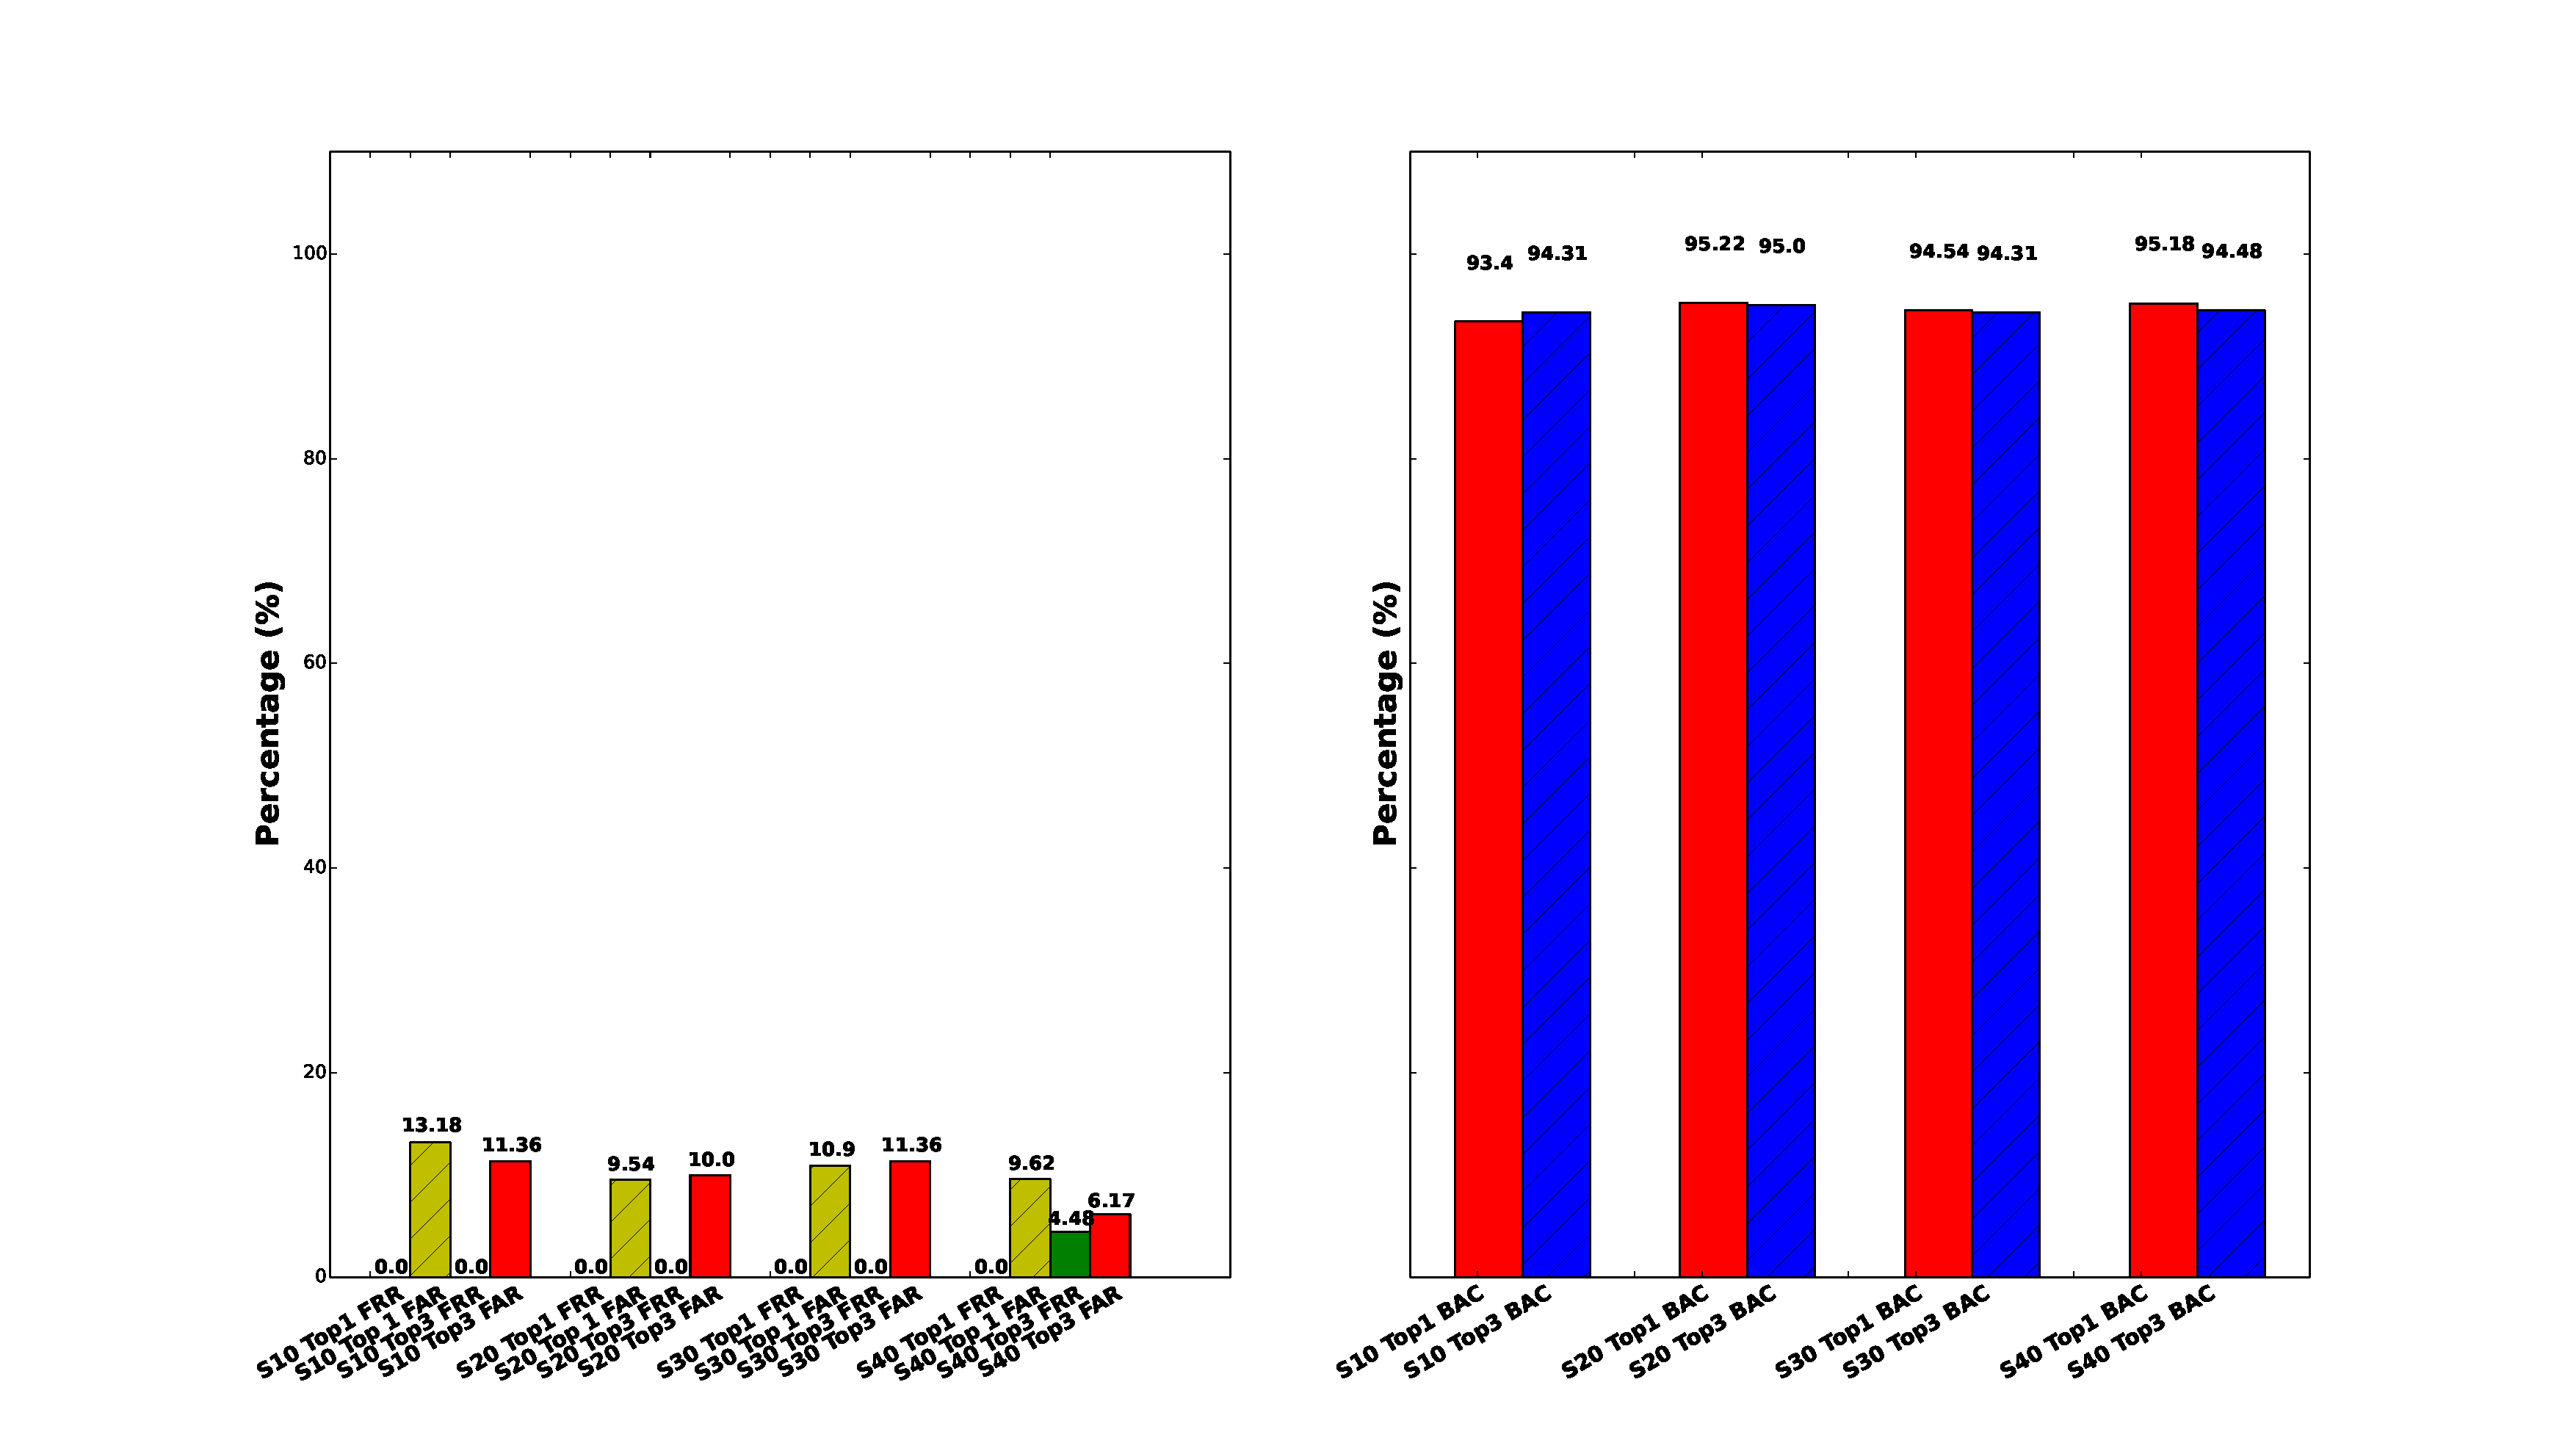
\includegraphics [width=.95\linewidth]{fig/exp1_vary_size_svm}
\caption{In this set of experiments, we studied whether the number of owner samples in the training set has a bearing on the SVM classification results. (a) shows the FRR and FAR results for each scenario, and (b) shows the BAC results.\label{fig:exp1_vary_size_svm}}
\end{figure*}

\vspace{4pt}\textbf{The Impact of Training Dataset Size:} Next we studied whether the number of owner samples in the training set has a bearing on the SVM classification results. We varied the number of owner training samples as 10, 20, and 30, and show the resulting FRR and FAR values in Figure~\ref{fig:exp1_vary_size_svm}(a) and BAC results in Figure~\ref{fig:exp1_vary_size_svm}(b). Note that we have in total 100 samples from the owner.

From the results, we observe that there is no clear trend when we vary the number of owner samples in the training set. When we increase the owner training samples from 10 to 20, the average BAC value increased, but only very marginally. This result suggests that to make the classification light-weight, thus suitable for wearable devices, we can use a small number of training set without hurting the performance.



\subsubsection{Thresholding-Based Classification}
\iffalse
\begin{table}[b]
\small
\begin{tabular}{|l||l|l|l||l|l|l|}\hline
& \multicolumn{3}{|c||}{2}& \multicolumn{3}{|c|}{3}\\\cline{2-7}
Sample duration (s)& FRR & FAR & BAC & FRR & FAR & BAC\\
&(\%) &(\%) &(\%) &(\%) &(\%) &(\%)\\\hline

Th Top 1                   & & &92.55 & & & 92.32  \\\hline
Th Top 3 Voting            & & &92.7 & & & 93.31 \\\hline\hline

& \multicolumn{3}{|c||}{6}& \multicolumn{3}{|c|}{10}\\\cline{2-7}
Sample duration (s)& FRR & FAR & BAC & FRR & FAR & BAC\\
&(\%) &(\%) &(\%) &(\%) &(\%) &(\%)\\\hline

Threshold Top 1                   & & & 93.71  & & & 94.69 \\\hline
Threshold Top 3 Voting            & & & 95.53 & & & 95.53 \\\hline

\end{tabular}
\caption{Average FAR, FRR, and BAC for Thresholding-based classification when we choose different 4 imitators in the training set (from the total 15 imitators). We have the results for different sample durations. In these results, we use the earliest 40 owner samples in the training set.\label{tab:kfoldfalse-th}}
\end{table}
\fi


\begin{table}[b]
\small
\begin{tabular}{|l||l|l|l||l|l|l|}\hline
& \multicolumn{3}{|c||}{2}& \multicolumn{3}{|c|}{3}\\\cline{2-7}
Sample duration (s)& FRR & FAR & BAC & FRR & FAR & BAC\\
&(\%) &(\%) &(\%) &(\%) &(\%) &(\%)\\\hline

Th Top 1                   &3.33 & 18.57&89.04 & 5.76& 16.63& 88.8  \\\hline
Th Top 3 Voting            &1.80 & 13.94&92.12 & 1.04& 12.67& 93.14 \\\hline\hline

& \multicolumn{3}{|c||}{6}& \multicolumn{3}{|c|}{10}\\\cline{2-7}
Sample duration (s)& FRR & FAR & BAC & FRR & FAR & BAC\\
&(\%) &(\%) &(\%) &(\%) &(\%) &(\%)\\\hline

Th Top 1                   &3.17& 8.74& 94.05 & 1.34& 1.99& 98.33 \\\hline
Th Top 3 Voting            &5.63& 9.15& 92.60 & 1.42& 4.78& 96.89 \\\hline

\end{tabular}
\caption{Average FAR, FRR, and BAC for thresholding-based classification when we choose different 40 owner samples in the training set (from the total of 100 samples).  We have the results for different sample durations. In these results, we use the first four imitators in the training set.\label{tab:kfoldtrue-th}}
\end{table}

\begin{figure*}[t]
\centering
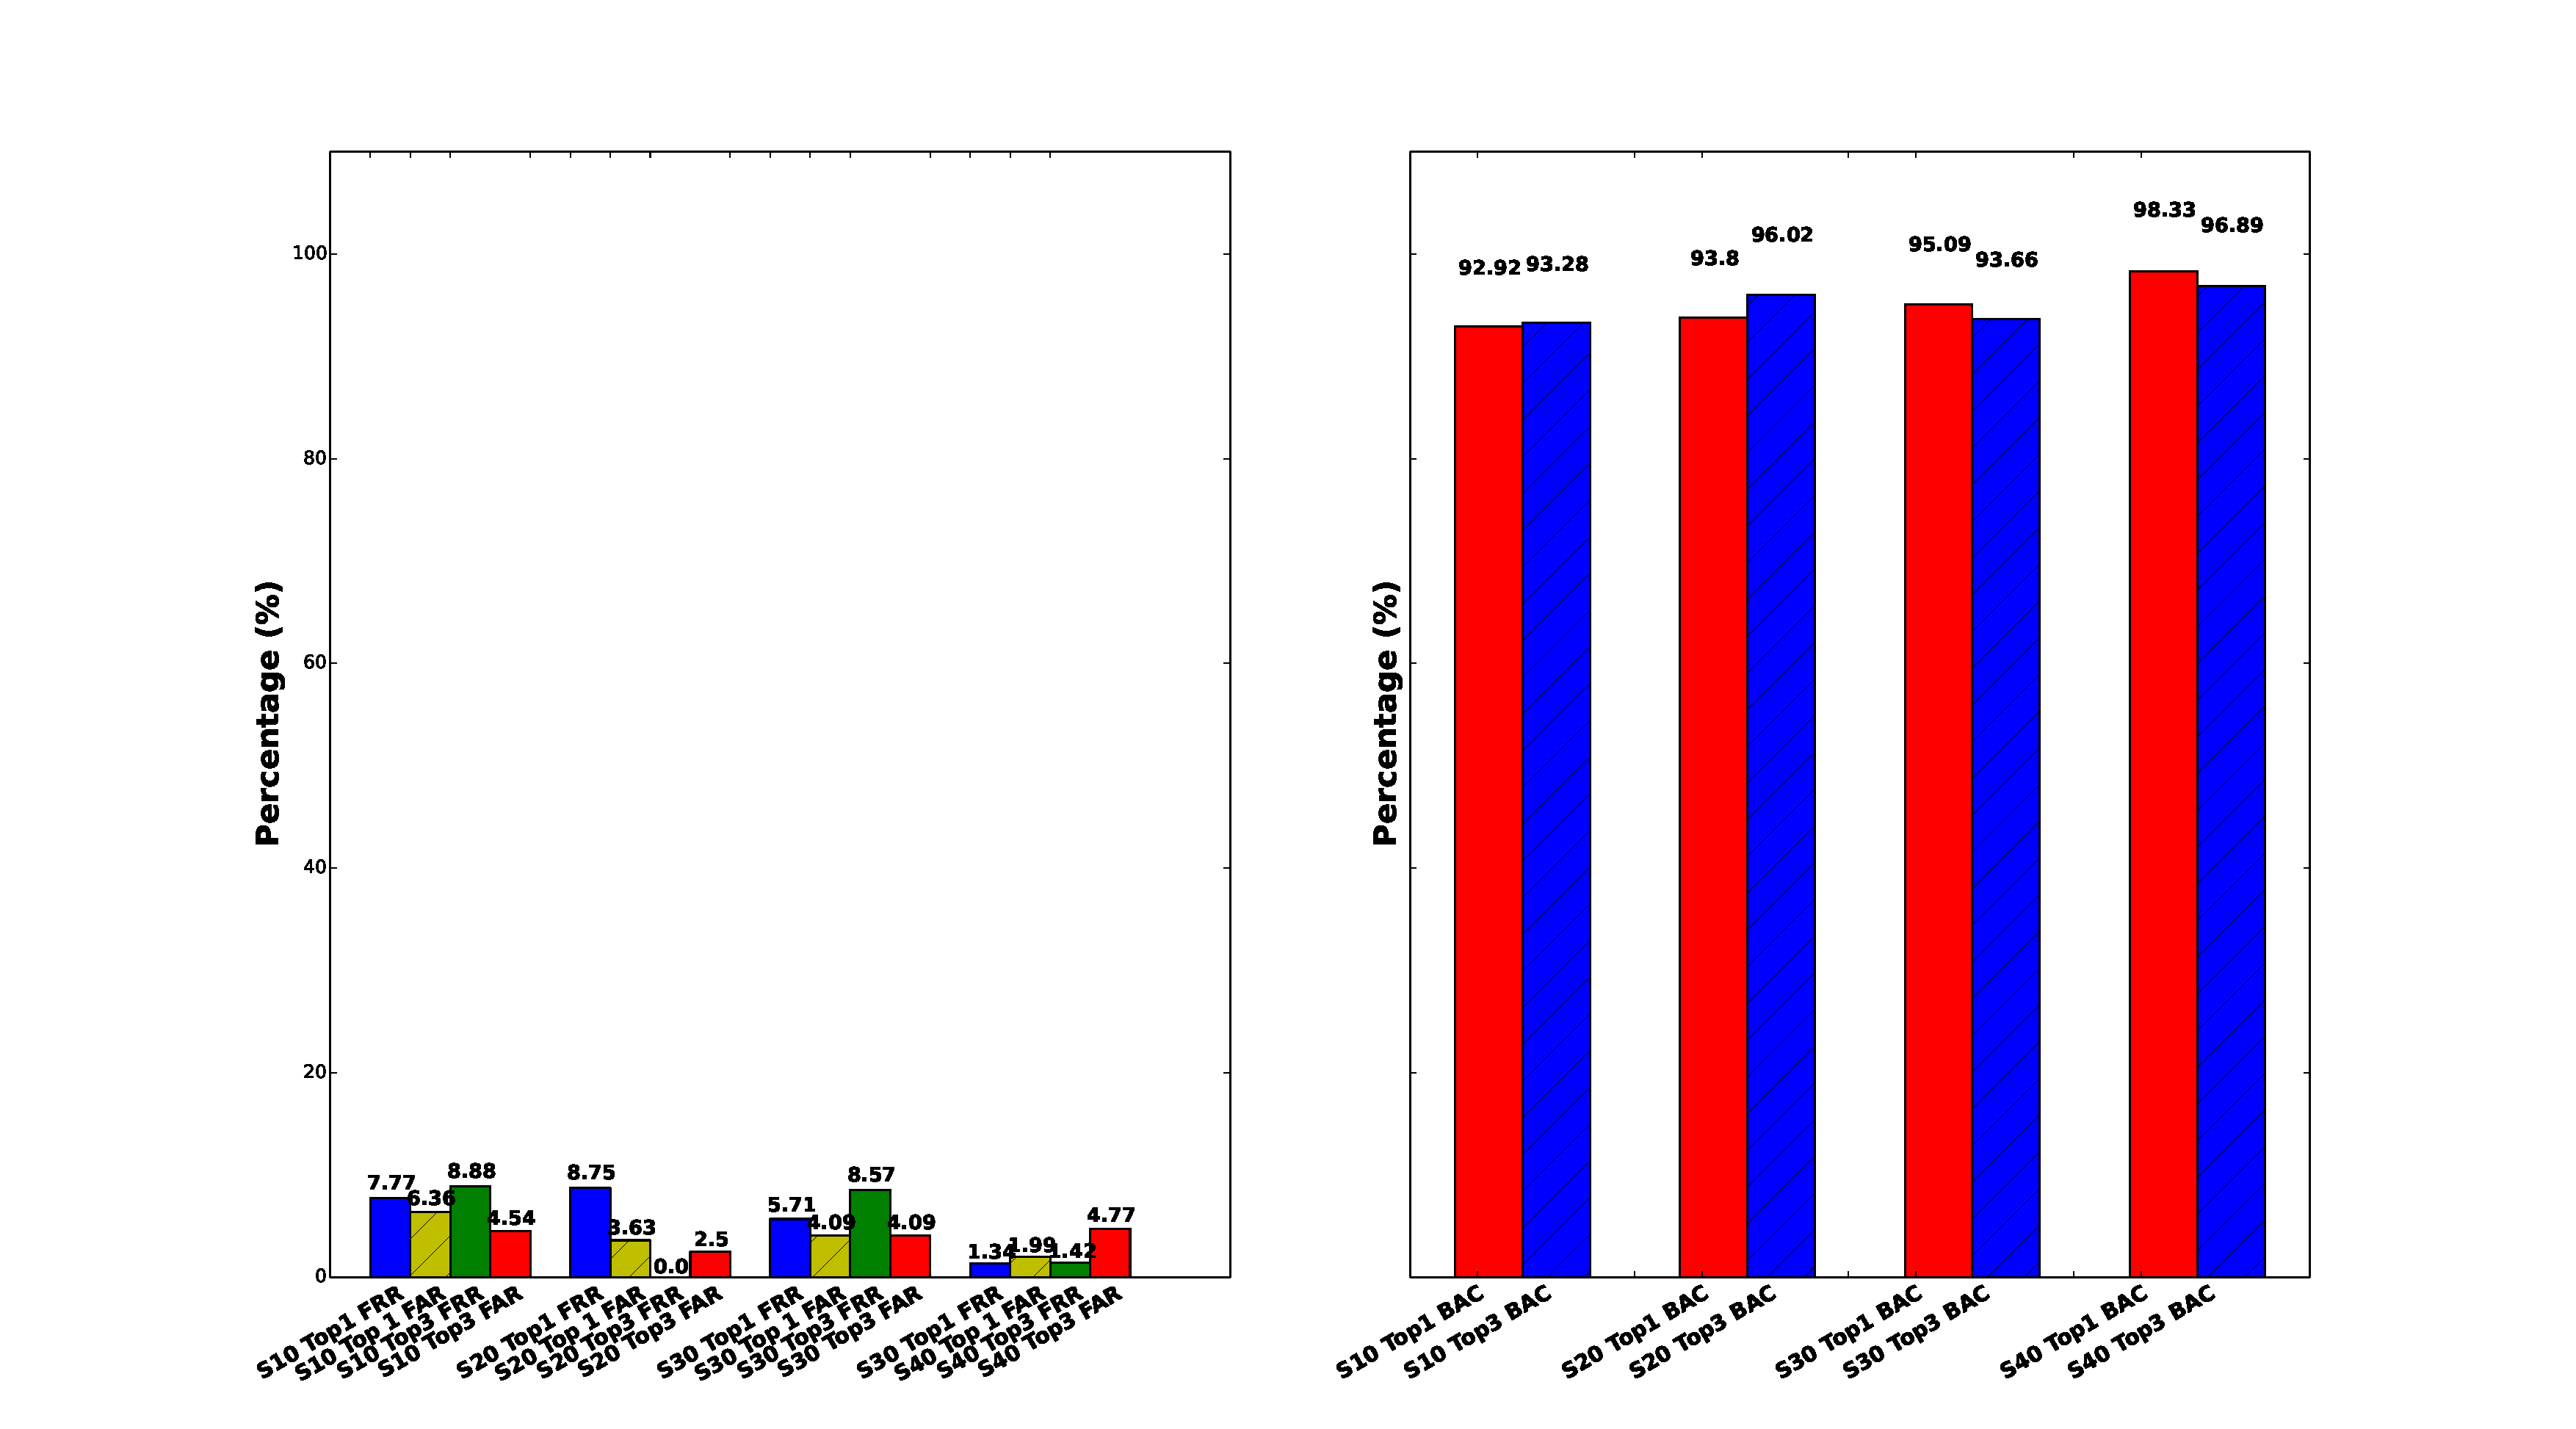
\includegraphics [width=.95\linewidth]{fig/exp1_vary_size_thre.eps}
\caption{In this set of experiments, we studied whether the number of owner samples in the training set has a bearing on the thresholding classification results. (a) shows the FRR and FAR results for each scenario, and (b) shows the BAC results.\label{fig:exp1_vary_size_th}}
\end{figure*}

\begin{figure*}[t]
\centering
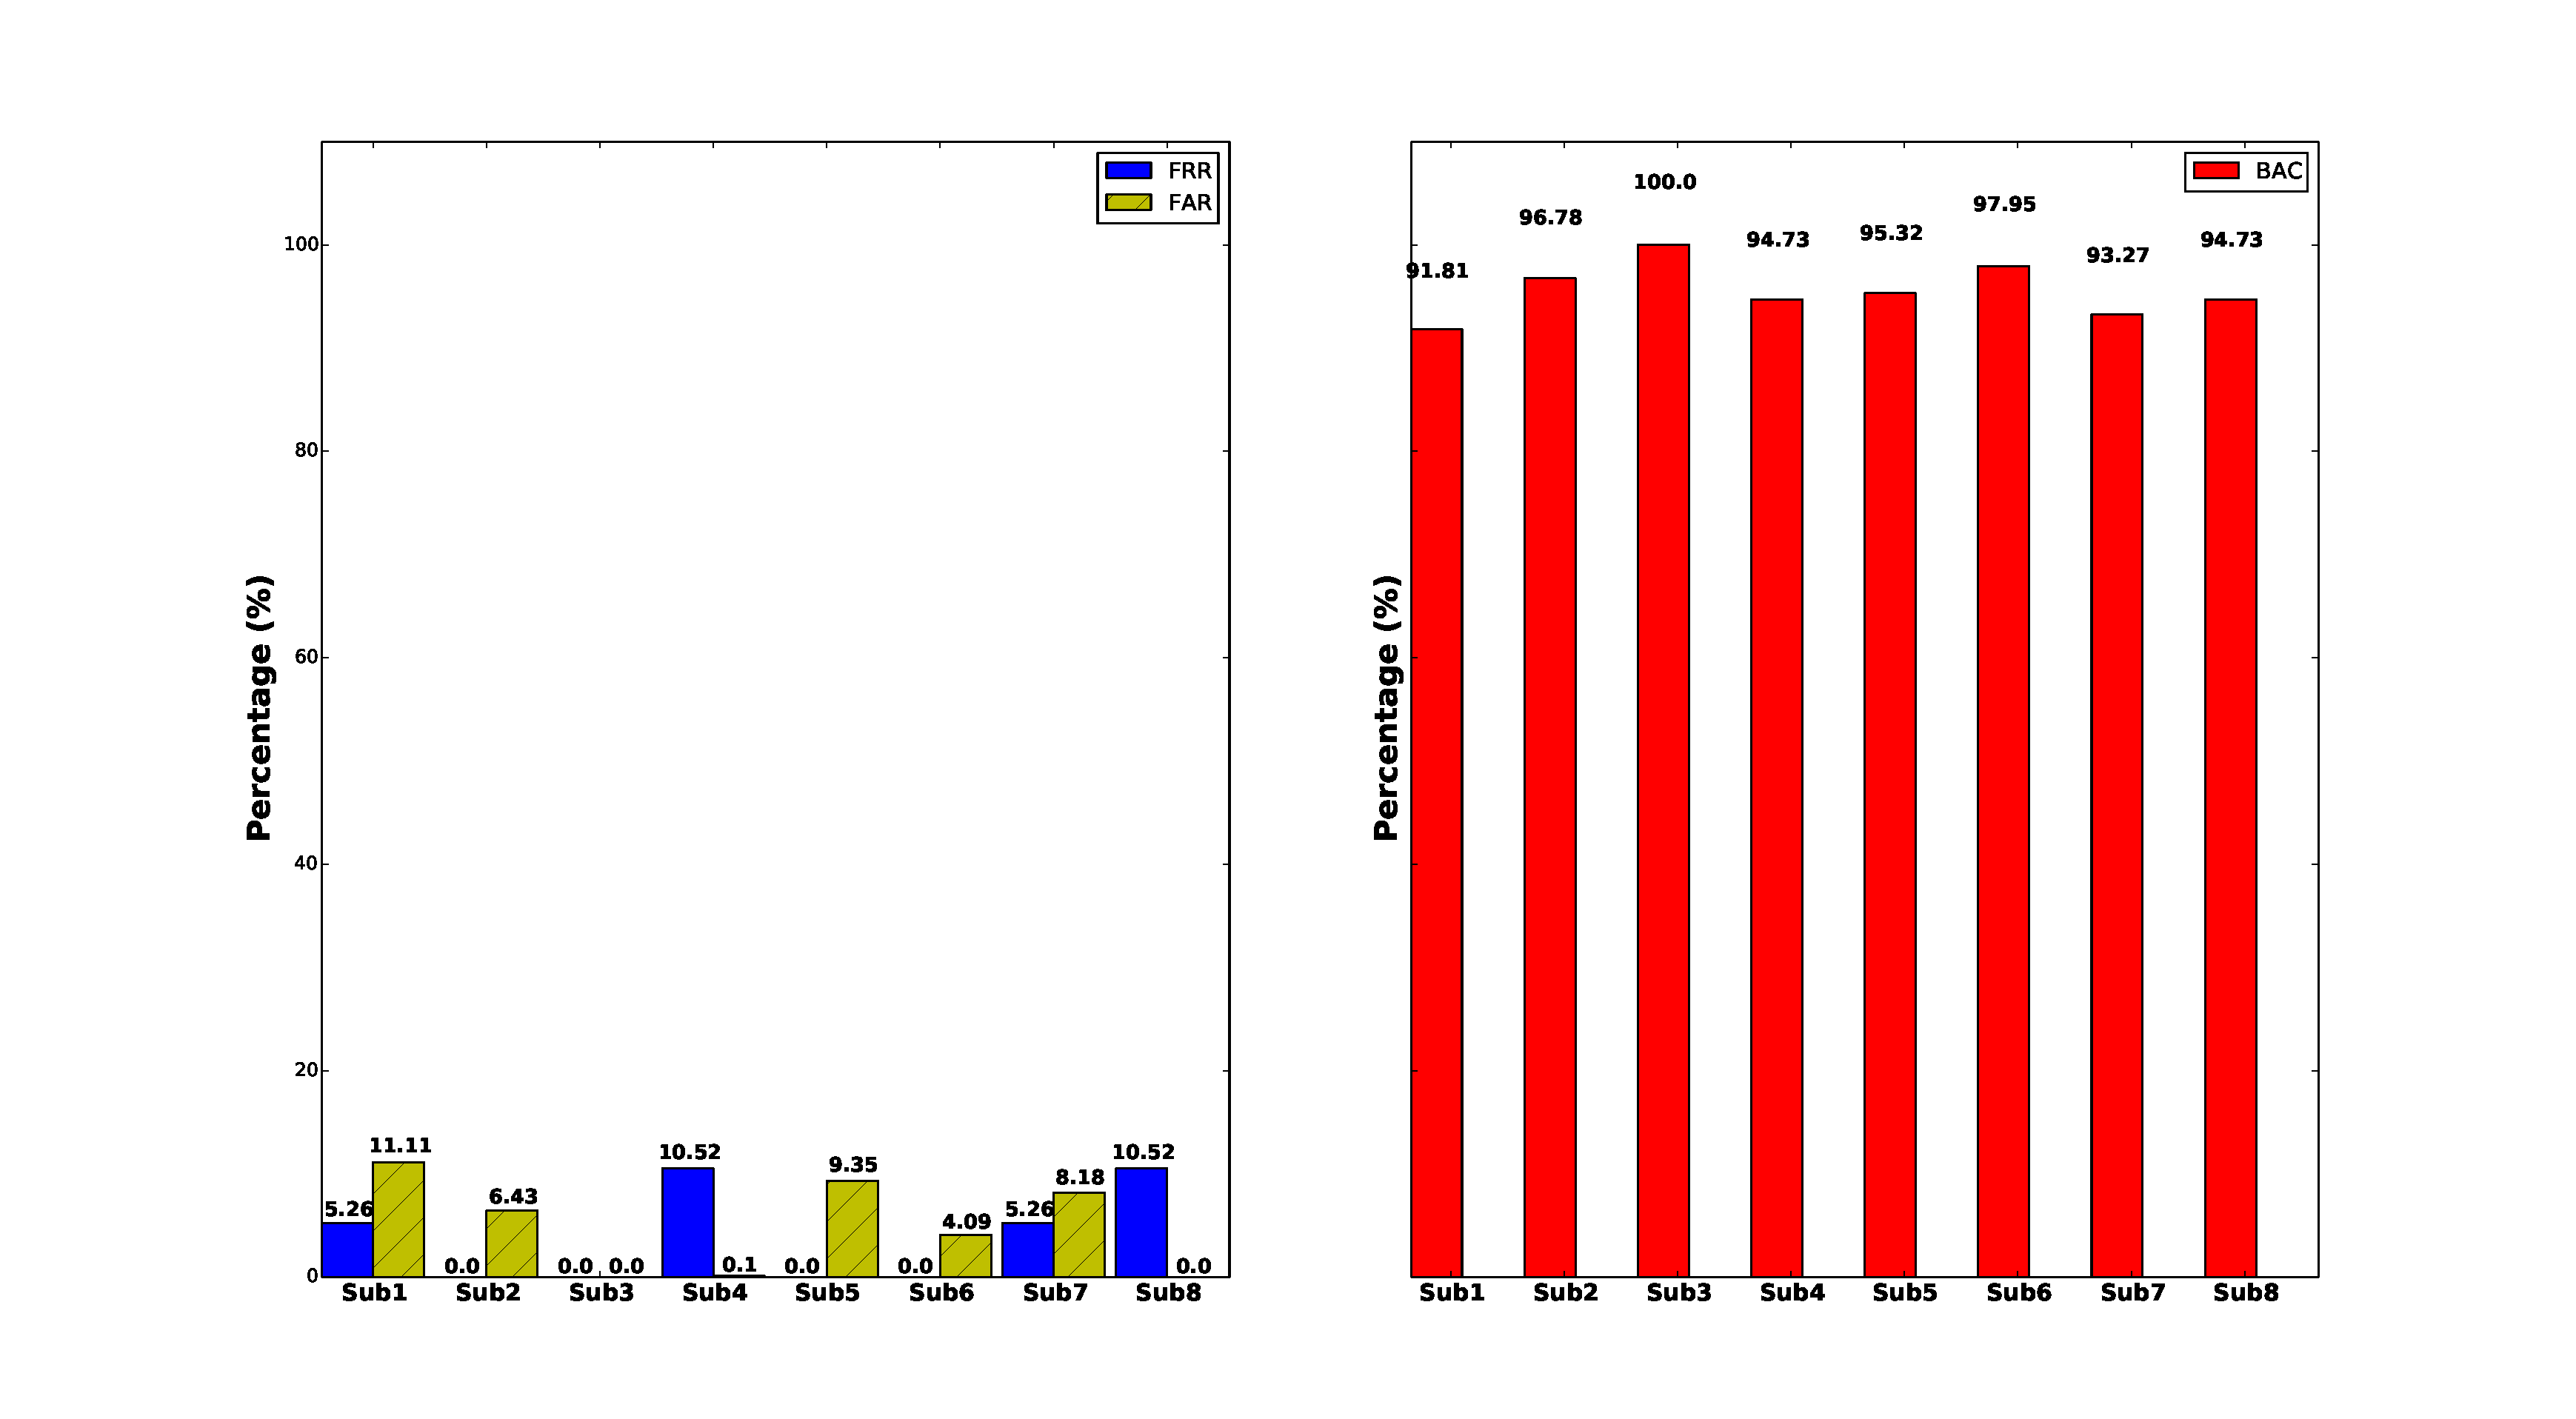
\includegraphics [width=.85\linewidth]{fig/exp2_frr_far_bac.pdf}
\caption{In this set of experiments, we studied whether a user can successfully repeat her own head-movement pattern. We had 8 subjects, each performing her own choice of head-movement patterns. We collected 38 samples for each subject. (a) shows the FRR and FAR results for each subject, and (b) shows the BAC results. Thresholding-based classification with top 3 voting was used to generate these results. \label{fig:exp2_frr_far_bac}}
\end{figure*}

Thresholding based classification only requires owner samples in the training set. In order to eliminate the impact of choosing certain training samples, we rotate the 40 training samples and summarize the average FAR, FRR, and BAC values in Table~\ref{tab:kfoldtrue-th}. Specifically, if we label the 100 owner samples as $S_1, S_2, ..., S_{100}$, then we ran 100 different experiments in this case, with training set being $\{S_1, S_2, ..., S_{40}\}$, $\{S_2, S_3, ..., S_{41}\}$, $\dots$, $\{S_{100}, S_1, ... S_{39}\}$, respectively.  Here, we also varied the sample duration: 2, 3, 6, and 10 seconds.

From Table~\ref{tab:kfoldtrue-th}, we have the following main observations:

\begin{enumerate}
\item \emph{Thresholding-based classification, though more light-weight, fares better than SVM.} Results in Table~\ref{tab:kfoldtrue-th} show that thresholding-based classification in general fares better than SVM (except the 6-second case). With 10-second sample duration, thresholding-based classification has a BAC value of 98.33\%. This is mainly because the thresholding-based classifier only relies on true training samples, hence more robust against imitators whose movement pattern is similar to that of the owner. This result is desirable because thresholding-based classification is much more light-weight than SVM classification, and thus more suitable for wearable devices.

\item \emph{For sample duration of 6 seconds or longer, comparing against the top 1 sample is sufficient.} We also observe that when the sample duration is 6 seconds or longer, it is preferred to compare the test sample against the top 1 training sample. This can significantly reduce the computation overhead of our system.

\item \emph{Thresholding-based classification has better FRR than FAR values.} Results in Table~\ref{tab:kfoldtrue-th} show that thresholding-based classification always has very low FRR values, even with short sample durations. With sample duration of 2 seconds, the FRR values are 3.33\% for top 1 testing and 1.80\% for top 3 voting, while the FAR values are 18.57\% for top 1 testing and 13.94 for top 3 voting. This suggests that even with short sample durations, thresholding-based classification is good at identifying the pattern of the same user. When the sample duration increases, we observe that the FAR values drop significantly, to as low as 1.99\% for top 1 testing and 4.78\% for top 3 voting for 10-second sample durations.
\end{enumerate}

\vspace{4pt}\textbf{The Impact of Training Dataset Size:} Next we studied whether the number of owner samples in the training set has a bearing on the thresholding classification results. We varied the number of owner training samples as 10, 20, and 30, and show the resulting FRR and FAR values in Figure~\ref{fig:exp1_vary_size_th}(a) and BAC results in Figure~\ref{fig:exp1_vary_size_th}(b). %***YZ: 40??***

Like the case in SVM classification, we didn't see any noticeable change in classification results with respect to the training data set size. This observation is advantageous in that we can reduce the training dataset size to further reduce the processing requirement and power consumption of our system.

\subsection{Head-movement Patterns are Repeatable}
In the second set of experiments, we would like to find out whether a user can successfully repeat her own head movement if each user is asked to come up with their own movement pattern.

\vspace{4pt}\textbf{Classification Results:} In this set of experiments, we had 8 subjects, and for each subject, we collected 38 $ACC$ samples with sample duration of 10 seconds. Each subject performed different head-movement patterns of their choice.

In generating the classification results, we employ a process that involves 8 iterations. In each iteration, we assume the legitimate glass owner is one of the users. We use 19 $ACC$ samples of this user as the training data set, and testing with his/her other 19 $ACC$ samples together with the other 7 user's $ACC$ samples. For each iteration, we calculate the resulting FRR, FAR, and BAC values (using the top 3 voting for thresholding-based classification), and show the results in Figure~\ref{fig:exp2_frr_far_bac}, where Figure~\ref{fig:exp2_frr_far_bac}(a) shows the FRR and FAR values, while Figure~\ref{fig:exp2_frr_far_bac}(b) shows the BAC values.



After carefully examining the results in Figure~\ref{fig:exp2_frr_far_bac}, we have the following main observations:
\begin{enumerate}
\item \emph{Head-movements are highly repeatable.} The first observation is that a user's head-movement pattern is usually highly repeatable. Among the 8 subjects that we studied, the highest BAC value is 100\%, and the lowest is 91.81\%, with the average BAC value of 95.57\%. Overall, this result suggests that the head-movement pattern is a promising biometric candidate for user authentication.

\item \emph{User head-movements have different level of stability.} Even from the small-scale 8 subject study, we found that users have different level of stability in their head-movements; some are much more stable than others. In our example, subject 3 has 0 FRR and 0 FAR, while subject 1 has 5.26\% FRR and 11.11\% FAR. We suspect that through proper training, subjects could improve their stability. However, we didn't test this hypothesis in this study. We also didn't notice any correlation between a user's stability with his/her age or gender.

\end{enumerate}

\begin{figure*}[t]
\centering
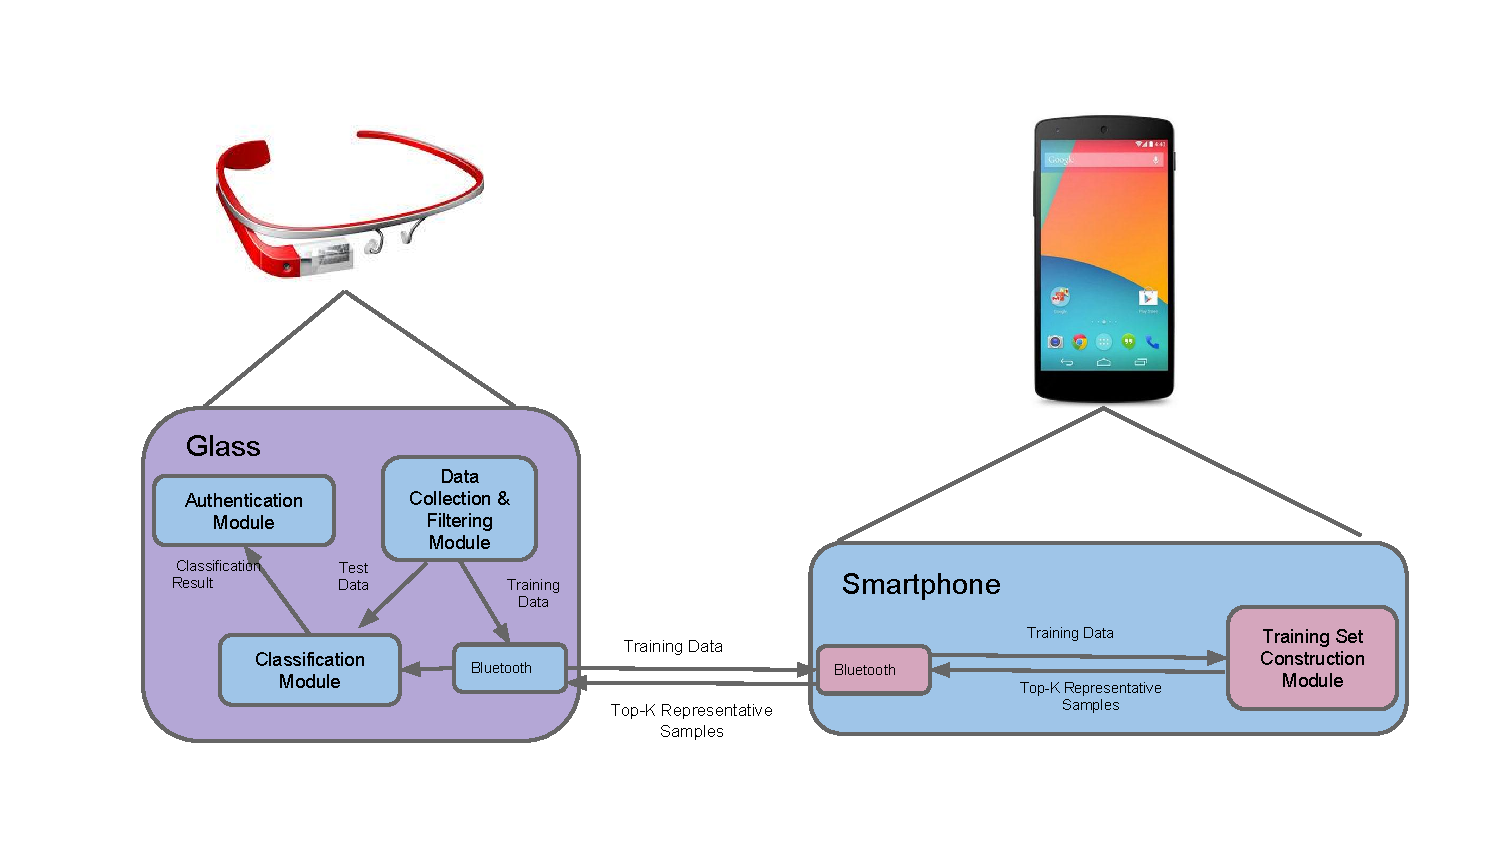
\includegraphics [width=.85\linewidth]{fig/sofware_architecture}
\caption{The software modules for the Headbanger authentication app. Note that the Training Set Construction Module is executed on the bluetooth-paired smartphone due to its computing intensiveness. \label{fig:software_arch}}
\end{figure*}


\subsection{Headbanger Authentication App Implementation}
We implemented the Headbanger authentication app on Google glass. Figure~\ref{fig:software_arch} shows the software modules the app consists of. Among all the software modules, the ``training set construction model'' is the most computing-intensive, and as a result, we executed the model on the bluetooth-paired smartphone. The rest of the modules are implemented and executed on the glass. In our on-glass app, the classification module runs the thresholding-based classification. Table~\ref{tab:glass} shows the measured processing latency (the time that elapsed between when the test sample is collected and when the authentication result is generated). The results show that even after our aggressive optimizations, the processing latencies are still rather substantial, which suggests that further optimizations are needed.

\begin{table}[b]
\small\centering
\begin{tabular}{|l|l|}\hline
sample duration (s) & processing latency (s) \\\hline
2 & 1.29 \\\hline
3 & 2.74 \\\hline
6 & 9.04 \\\hline
10 & 2.48 \\\hline
\end{tabular}
\caption{Measured processing latencies on Google Glass with different sample durations. We generated the results using Top 1 testing for thresholding based classification.\label{tab:glass}}
\end{table}



\iffalse
\subsection{Controlled Experiments: Can You Repeat Your Body Movement?}\label{sec:experiment1}
We first investigate the consistency of the movement performed by each subject. Physical biometric such as fingerprint and iris, which are permanent characteristics that remains regardless environment, emotion, and time. However, behavioral biometric is combined with human controllable movement
\fi


\section{Discussion}\label{sec:disc}

In this study, we showed that head-movements have the potential to be used as
a reliable behavioral signature for user authentication.
We will now discuss some of the limitations that we identified from this work
and prospects for future work as below.

\iffalse
\subsection{Reliability}
Our work in this paper shows that head-movements are distinctive and
repeatable in controlled settings. However, in reality, the behavior of
head-movement signatures over chaotic settings will be a key factor to decide
on the effectiveness of this approach. Our work only evaluates the case when a
user is in a stationary setting when attempting to login, such as when sitting
on the chair or standing still. The performance of this approach in realistic
mobile settings such as walking or in a vehicle is yet unknown. It is also
unclear if the head-movement patterns are repeatable in such a mobile environment, or
if the ambiguities of vehicle motion versus head-motion can be separated. 
%%For example, we don't know whether a person's
%%head-movement signature will be the same no matter whether she is sitting,
%%standing still, walking, running, or driving.
%%The most important concern is the reliability of human head-movements. Even
%%though we have shown that head-movements are rather distinctive and
%%repeatable
%%in a controlled setting, it is yet unclear how it will perform in realistic,
%%but chaotic settings. For example, we don't know whether a person's
%%head-movement signature will be the same no matter whether she is sitting,
%%standing still, walking, running, or driving.
Similarly, a person's head-movement signature may also depend on the mood/energy level of
the person; for example, a fresh and energetic user may provide significant
head-movements as compared to a sick or tired user whose signatures may not
even be detectable. Inconsistencies in the accelerometer sensor such as drift and temporal bias can
significantly affect the nature of inferred head-movement signature.
Head-movements, on the other hand, may also evolve over time for a person
which call for periodic calibration of the system and/or the training data.
%To address these two temporal changes, we may need to periodically
%recalibrate
%the sensors and dynamically adjust our training data to reflect new movement
%trends.
While reliability metric was out of the main scope of this paper, we are keen
to address the same in future work.
\fi

\subsection{Power consumption}

\begin{table}
\centering
\begin{tabular}{lccc}
\hline
Component    & Power Consumption (mW) & Duration (s)       \\ \hline\hline
Sensor  & 29                    & 10       \\
Speaker & 410                    & 10      \\
CPU      & 1600                   & 14.4 \\ \hline
\end{tabular}
\caption{Power consumption on Google Glass of components relevant to 
\systemname.  The CPU (running at 
maximum frequency) power consumption includes that of the heads-up display 
screen being ON as well. Duration marks the time for which
component was ON during the a 10 sec music cue length trial}
\label{tab:pow}
\end{table}

Google Glass is an example of a wearable device that is heavily battery power 
constrained. Measuring the power consumption of the Glass's battery is a 
challenging task as that requires physically dismantling the device. 
We refer to the measurement paper on Google Glass by Robert et. 
al~\cite{likamwa2014draining} for the power consumption of the 
key components relevant to \systemname~implementation on Glass: the speaker 
for music cue playback, the accelerometer sensor and the CPU being ON during 
the entire authentication process. We report the relevant numbers in 
Table~\ref{tab:pow}. While the high CPU power consumption may not necessarily 
be surprising, the speakers also extrude considerable energy from the battery. 
We note that one possible solution for future consideration would be to play 
the music cue as intermittent notes over the duration, for example a ping or a 
beat sound periodically, where the speaker would be switched ON only during 
playback.

\subsection{Is this secure?}
An authentication system must have an effective protocol ensuring security of 
the authenticating user's data. Our system runs an implicit
authentication protocol where the user is given a finite set of (calibrated) 
music tracks to pick, based on which the user makes head-movements that are 
used as unique signatures for authentication.
Our design assumes implicit security of the user's data, as a
user voluntarily accepts the enforcement of conducting head-movements  
in response to the music. It is arguable that such enforcements are an 
integral part of most commonly used authentication systems; for example, 
typing a password, swiping the finger on the fingerprint sensor, approving of 
the camera recognizing the face. In all these cases the user is aware 
that he/she is inputing data into the system for authentication.

One way of compromising security would be a successful spoof of the 
head-movement by an adversary. For example, head-movements from an authorized 
user may be imitated by an adversary attempting to login to the device. 
%However, this requires that the wearable device is physically accessible to 
%the adversary. Since head-worn devices are at the visual field of view of the 
%user the chances of it getting lost or being stolen will be lower than other 
%wearable devices such as smart-watch or smart-necklaces. 
If the head-movements from the user is regular (such as a nod), it may be 
easily imitated as opposed to a random head-shake such as a head-bang.
To understand the effect of imitation on the accuracy of authenticating a user 
to \systemname, we conducted an experiment (under the same set up as  
described in section~\ref{sec:results}) where 29 volunteer participants 
were asked to imitate the head-nod movements of one user (one of the authors) 
who was trying to authenticate to the device using a 10 sec music cue. A total 
of 30 trials were conducted of which 10 samples were used as test data and 20 
for training. Our evaluations of this dataset resulted in reasonable accuracy 
values of, an 
EER of 7.2\% and a balanced 
accuracy $BAC = 1 - ((FAR+FRR)/2)$ of 94.5\% for the authorized user. Our 
results indicate that attacking the system through imitation of a simple 
head-gesture can still be challenging.

%A seamless design
%would ensure that the system captures even the slightest of the subconscious
%head-movements in the event that the user does not make any enforced
%head-movements. In such cases the head-movement signatures will have to be
%much more elaborate with multiple attributes that correspond to the different
%realistic use-cases of the system.

\subsection{Multi-Modality}
Inconsistencies in the accelerometer sensor such as drift and temporal bias can
significantly affect the nature of inferred head-movement signature.
Head-movements, on the other hand, may also evolve over time for a person
which call for periodic calibration of the system and/or the training data.
The array of motion sensors (accelerometer, gyroscope, inertial measurement 
unit) open up opportunities for multi-modal motion sensing. For example,
in Glass, accelerometer data can be combined with gyroscope measurements to 
provide multi-dimensional head-movement features that can improve the quality 
of the inferred signatures. Head movements can also be combined with other 
body movements to generate valuable, reliable signatures for authentication. 
%Additionally, head-movement is just one type of body movements, and we can
%investigate other types of body movements as well.
For example, through a simple test experiment using the Google Glass
infra-red (IR) light sensor (we had to root the Google Glass to access the
IR sensor unit) we observed that the blinking and winking patterns of users in
response to the music stimulus were reasonably differentiable among users.
Such patterns may also independently serve as another biometric that can be
used for authentication purpose, or can be combined with head-movements for better results.
Recent studies have shown that heart beat or pulse can also serve as reliable
biometric for authentication purposes~\cite{hernandezbioglass,nymi}.
We reserve such potential enhancements to our system for future implementation.
%A recent study has shown that Google glass can detect human heart
%beat~\cite{hernandezbioglass}; heartbeats can thus be
%used as another biometric.
%If extra hardware can be introduced, then more movement patterns,
%such as eye movement, can be leveraged as well.

\iffalse
\subsection{Seamless Protocol}
An authentication system must have an effective protocol for authenticating
users seamlessly to their device. Our system runs a simple authentication
protocol where the user is given a finite set of (calibrated) music
tracks to pick, and based on which the user makes head-movements in response.
Our design assumes that the user voluntarily accepts the enforcement of the
requirement of head-movements in response to the music. A seamless design
would ensure that the system captures even the slightest of the subconscious
head-movements in the event that the user does not make any enforced
head-movements. In such cases the head-movement signatures will have to be
much more elaborate with multiple attributes that correspond to the different
realistic use-cases of the system.
%Our protocol can consist of several steps. In the first step, the user will
%be
%asked to choose a user name from all the legitimate users of the device.
%Then,
%the user will be asked to select the favorite music track of the claimed
%user.
%If the selection is correct, the device will play the music and ask the user
%to move along (including head movement, eye blinking/winking, etc). ***YZ:
%what else??? ***
\fi

\iffalse
\subsection{Processing/Battery Power Constraints}
Battery power consumption and computing power are very important parameters
for consideration when optimizing a design to accommodate to wearable devices.
Wearables usually have serious resource limitations, especially in terms of
processing power and battery power.
This paper, addresses these concerns through optimization strategies in the
head-movement signature classification stage of the proposed authentication
algorithm. For wearables it is important that such optimization strategies are
taken to next levels until a roadblock is reached.
%In this paper, we have considered a set of
%optimization techniques to reduce the processing demand as well as power
%consumption, e.g., testing against top $K$ samples instead of  the entire
%training set, using thresholding-based classifier instead of SVM classifier.
For example, one such strategy extension in this work can be that, after a
short duration, before the entire music is played, if it is found that a
user's movement does not match the signature of the claimed user
with sufficient confidence level, then the on-site classification may be
terminated  instead of waiting for the entire duration to yield the rejection.
Another example, may include cyber-foraging strategies to offload heavy
computation tasks, such as classification, to the user's Bluetooth paired
smartphone.
\fi

\subsection{Large Scale User Study}
To be adopted as a primary authentication mechanism on smart-glass devices,
the technique will have to be evaluated over a large number of usage and
and over a large user base. Conducting such rigorous large-scale experiments
is typically infeasible in academic laboratory settings. We reserve such
large scale experiments for future work, and hope to accomplish through
industry collaborations. We will, however, be releasing our data-sets to the 
public in the near future.
\section{Related Work}\label{sec:related}
Headbanger is a behavioral biometric based
authentication system, which focuses on head movement. 
%To our best knowledge, it is the first wearable authentication system that 
%only relies on accelerometer signatures from human \emph{head} motion. 
Below, we review the related literature on mobile device authentication.

%in wearable/mobile device based schemes, infrastructure based
%schemes, and biometric-rich based schemes.

%\subsection{Wearable/mobile device based schemes}
The work by Harwin et al.~\cite{harwin1990analysis} is usually considered the 
first to propose use of head gestures by combining pointing and movements
for human computer interaction. 
In~\cite{westeyn2004recognizing}, the authors used 
eye-blinking pattern as a unique feature for
authentication. They achieved 82.02\% accuracy with 9 participants. Compared 
to eye blinking pattern, head-movements can provide much more entropy, 
therefore can be considered as a more suitable biometric characteristic. 
The work by Ishimaru et al.~\cite{ishimaru2014blink} comes close to our system 
design; they proposed to combine the eye blinking frequency from the infrared 
proximity sensor and head motion patterns from accelerometer sensor on Google 
Glass to recognize activities (e.g., reading, talking, watching TV,
math problem solving) 
The key difference of our approach from ~\cite{ishimaru2014blink} is 
that, their approach focused on common head-movement and eye-blink patterns 
when people employ the same activities such as reading, typing, etc. 
We carefully investigated the head-movements from human subjects and found 
that they are unique to each person. 
Our system also identified these head-movements with a higher accuracy (95$\%$ 
versus 82$\%$ in ~\cite{ishimaru2014blink}).

There are also a number of physiological activity recognition studies 
using computer vision~\cite{kjeldsen2001head,hernandezbioglass}. 
While~\cite{kjeldsen2001head} primarily uses computer vision to detect 
head gestures, BioGlass~\cite{hernandezbioglass}
combines Google Glass's accelerometers, gyroscope, and camera to
extract physiological signals of the wearer such as pulse
and respiratory rates. Camera processing on wearable devices, especially 
Google Glass is compute intensive and has a high energy 
budget~\cite{likamwa2014draining}.

Accelerometers have long been used to sense, detect and also recognize
movements in other parts of the body; for example, gait recognition requires 
sensing in areas such as waist~\cite{ailisto2005identifying},  
pocket~\cite{gafurov2007gait}, arm~\cite{okumura2006study,gafurov2008arm},
leg~\cite{gafurov2006biometric} and ankle~\cite{gafurov2011user}.
These techniques, though well known, may not be suitable for on wearable 
devices due to complexity (computation and energy) in the machine learning 
process.
%They are similar in that they collect the raw accelerometers data
%and apply signal processing and/or machine learning techniques  to perform
%authentication.

Hand gesture and touchscreen dynamics are often coupled for
authenticating to a (touchscreen) device. A number of contextual features
including biometrics~\cite{sae2012biometric} (e.g. finger length, hand size,
swipe/zoom speed, acceleration, click gap, contact size, pressure)
and behavioral feature (e.g. touch location, 
swipe/zoom length,
swipe/zoom curvature, time, duration) have been exploited as
effective features for authentication 
purpose~\cite{frank2013touchalytics,cai2013mobile,feng2014tips}.
While most of the techniques require users to explicitly conduct a
gesture following a specific pattern, TIPS~\cite{feng2014tips}
proposed a multi-stage filtering with dynamic template adaptation
strategy to perform the user authentication in uncontrolled
environments -- when a users naturally their phone. 

There is indeed a significant prior art in authentication system 
implementations using various techniques such as 
speech~\cite{reynolds2000speaker}, computer vision and image
~\cite{bowyer2006survey}, graphical passwords~\cite{biddle2012graphical}, 
gestures~\cite{sherman2014user}, biometric 
fingerprints~\cite{jain1997identity}. 
In this paper, we do acknowledge the viewpoint that our approach can also be 
used as a complementary scheme to most of the existing techniques in the 
authentication application space.

%It was extended by Kjeldsen~\cite{kjeldsen2001head} to more
%categories such as continuous control, spatial selection and
%symbolic selection

%Gafurov et al.~\cite{gafurov2006biometric} developed a wearable
%biometric gait authentication system. The sensor is attached to the
%lower leg to extract the gait patterns -- accelerations in three
%directions: vertical, forward-backward and sideways motion of the
%lower leg. A combination of these accelerations is used for
%authentication. ~\cite{gafurov2011user} ankle
%\subsection{Infrastructure based schemes}

%\subsection{Biometric-rich based schemes}
%Fingerprints

% are we the first one? the cloest work? how far we are going to reach out? categories in general: image? voice? touch?
% on glass; body movement;

%mobisys 2014 papers

%gesture based authentication

%Music based movements -- GaTech

%Japanese paper on google glass and eye-wink

%hardware fingerprinting -- check CCS 2014

%acc-based authentication
%http://ieeexplore.ieee.org/xpl/articleDetails.jsp?arnumber=5634532&sortType%3Dasc_p_Sequence%26filter%3DAND%28p_IS_Number%3A5634461%29

%wearable security
%http://gaia.cs.uiuc.edu/papers/wss.pdf

%commercial solutions: Nymi -- eyewink blink pattern

%BioNym -- heartbeat

\section{Concluding Remarks and Future Direction}
\label{sec:conc}
As wearable devices are increasingly weaved into our everyday life, providing security to the data acquired by or accessed through these devices becomes critically important. In this study, we have developed a user authentication system that uses head-movement patterns for direct
authentication to a wearable device. Compared to existing authentication solutions, the proposed solution delivers accurate authentication, is robust against imitation attacks, incurs low processing delays, and offers great convenience to users.

%We developed a light-weight approach that
%infers head-movements of users in response to music and generates signatures
%that are unique to every user.
%Our technique specifically uses the dynamic time-warping (DTW) tool to
%generate a head-movement feature that contains the mean and standard
%deviation of the DTW score of each user, determined over a multiple-user data
%set. The matching is conducted based on a thresholding scheme.
%Experimental observations revealed that the head-movement signatures generated
%using the dynamic time-warping tool, in response to the same music track, were
%consistent in typical stationary environments such as user sitting or
%standing at one location while attempting to authenticate. We leveraged the
%consistency in the head-movement signatures to develop two classification
%algorithms, based on machine learning and adaptive thresholding, to
%efficiently and accurately label user signatures.
Through an extensive evaluation that involves 95 users, we observe that the
average true acceptance rate of our approach is at 95.57$\%$ and the false
acceptance rates at 4.43$\%$. We also observe that even simple head-movement patterns only allow less then 3\% of the imitation attacks to succeed. We have also implemented an app on Google Glass, and measured the end-to-end processing delay of less than 2 seconds for a 10-second data sample. As a result, we believe it is realistic for the proposed authentication system to be executed on resource-constrained devices such as smart-glass. We further believe the proposed method can help enable wider deployment of wearable devices and apps in our life. Towards this goal, in our future work, we will focus on how to make the head-movement based user authentication approach more reliable in real-world settings.

%We have also optimized our algorithms to
%minimize the processing latencies and power consumption, making them suitable
%for wearable devices.
%The multi-user data sets were validated and verified during the
%course of our evaluations and will be released for public use in near future.

\iffalse
In this paper, we present the design, implementation and evaluation
of Headbanger, a head gesture based authentication system.
Headbanger generates a signature from user's head-movements in
response to short duration of audio track with fast beats, and uses
this signature as the behavioral biometric for authentication.
Through extensive experiments on the prototype on Google Glass
involving ?? users, we demonstrated that Headbander can achieve **\%
accuracy and thus with proper audio stimuli, head-movement alone
will be reasonably sufficient to serve a effective behavioral
biometric for authentication. We believe this work will be the basis
for using audio catalyst to enrich more useful human contextual
applications.
\fi 

\balance
%\scriptsize
%\footnotesize
%\small
%\bibliographystyle{acm-sigchi}
\bibliographystyle{abbrv}
\bibliography{sugang}
\end{document}
